\documentclass[10pt,fleqn,twoside]{book}
\topmargin=3cm

%cambiar fuente defecto
\usepackage{helvet}
%\renewcommand{\normalfont}{\sfdefault}

\usepackage{amsmath, amsfonts, psfrag, fancyhdr, layout, appendix, subfig}
\usepackage{graphicx}

\usepackage{ucs}
\usepackage[utf8,utf8x]{inputenc} %codificacion documento
\usepackage[spanish]{babel}
\usepackage{makeidx}
%\usepackage{ucs}

%imagenes donde deben ir
\usepackage{float}

\usepackage{color}

\definecolor{lightgray}{rgb}{0.83,0.83,0.83}
\definecolor{darkgray}{gray}{0.40}

%Colores predefinidos para usar con listing
\definecolor{code_fg}{RGB}{50,50,50}
\definecolor{code_bg}{RGB}{240, 255, 225}
\definecolor{code_coment}{RGB}{0, 80, 0} 
\definecolor{code_keyword}{RGB}{0, 50, 100}
\definecolor{code_indetif}{RGB}{0, 128, 255}
\definecolor{code_number}{RGB}{80, 80, 80}
\definecolor{console_bg}{RGB}{0, 79, 117}
\definecolor{console_fg}{RGB}{250, 250, 250}
\definecolor{console_key}{RGB}{0, 79, 157}

%color de los enlaces
\definecolor{link}{RGB}{0, 79, 157}


%This change labels of subfig
\renewcommand{\thesubfigure}{\alph{subfigure}\arabic{subfiggroup}}
\captionsetup[subfigure]{labelformat=simple,labelsep=colon,
                         listofformat=subsimple}
%\captionsetup{lofdepth=2} This is in order to list the subfigures in the LOF
\makeatletter
 \renewcommand{\p@subfigure}{}
  %Esto lo agrego yo para tener subfiguras a1, b1, ... a2, b2, ... 
  %Se reinicia cada vez que una nueva figura es convocada (como es debido).
  \newcounter{subfiggroup}[figure] 
\makeatother

\usepackage{epsfig}

%Esto genera enlaces en el PDF
\usepackage{url}

%cambiar margenes
\def\changemargin#1#2{\list{}{\rightmargin#2\leftmargin#1}\item[]}
\let\endchangemargin=\endlist


% \usepackage{html}
%Esto es para el conversor latex2html


%Definición de margenes
\usepackage[left=4.5cm,top=3cm,right=2cm,bottom=2.5cm]{geometry}
\sloppy
\pagestyle{empty}

% Code for creating empty pages
% No headers on empty pages before new chapter
\makeatletter
\def\cleardoublepage{\clearpage\if@twoside \ifodd\c@page\else
    \hbox{}
    \thispagestyle{plain}
    \newpage
    \if@twocolumn\hbox{}\newpage\fi\fi\fi}
\makeatother \clearpage{\pagestyle{plain}\cleardoublepage}

% Code for creating fully-empty pages
% Fully empty pages before command is called
\makeatletter
\def\clearfullypage{\clearpage\if@twoside \ifodd\c@page\else
    \hbox{}
    \thispagestyle{empty}
    \newpage
    \if@twocolumn\hbox{}\newpage\fi\fi\fi}
\makeatother \clearpage{\pagestyle{empty}\clearfullypage}

% Dutch style of paragraph formatting, i.e. no indents.
\setlength{\parskip}{1.3ex plus 0.2ex minus 0.2ex}
\setlength{\parindent}{0pt}


% Double space for REVISION
%\renewcommand{\baselinestretch}{2.0}

%Print subsubsection numbers and put them in TOC
\setcounter{secnumdepth}{3}
\setcounter{tocdepth}{3}

\makeindex

%enlaces web en pdf remplazado por url
\usepackage{hyperref}

\hypersetup{
    colorlinks=true,
    linkcolor=black,
    urlcolor=link
}


%listings reconoce la sintaxis de varios lenguajes y permite otras configuraciones.
\usepackage{listings}
%listing definicion para formateo de codigo fuente
\lstdefinestyle{Python}
{
    basicstyle=\small\ttfamily\color{code_fg},
    backgroundcolor=\color{code_bg},
    keywordstyle=\color{code_keyword}\tt, % underlined bold black keywords
	identifierstyle=\color{code_indetif}, % color identificadores
	commentstyle=\color{code_coment},                       % comentarios
	stringstyle=\ttfamily,                                 % typewriter type for strings
	showstringspaces=false,
	frame=shadowbox,%\linewidth=3,
	framexleftmargin=8mm,
	rulesepcolor=\color{code_fg},
	backgroundcolor=\color{code_bg},
	language=Python, 
	numbers=left, 
	numberstyle=\color{code_number}\footnotesize\tt,		%estilo numero linea
	tabsize=4, 						                        %tamaño tabulacion 	    
	%showspaces=true,
}

\lstdefinestyle{HTML}
{
    basicstyle=\small\ttfamily\color{code_fg},
    backgroundcolor=\color{code_bg},
    keywordstyle=\color{code_keyword}\tt, % underlined bold black keywords
	identifierstyle=\color{code_indetif}, % color identificadores
}

\lstdefinestyle{consola}
{
    basicstyle=\ttfamily\color{console_fg},
    backgroundcolor=\color{console_bg},
}


%FIN Definicion para Formateo Codigo

\usepackage{lmodern}% http://ctan.org/pkg/lm 

\begin{document}


%Cambiar Cuadros por Tablas y lista de... Debe ir después de \begin{document}
%\renewcommand{\listtablename}{Índice de tablas} 
%\renewcommand{\tablename}{Tabla} 


\pagenumbering{arabic}

%%%%%%%%%%%%%
\frontmatter
%%%%%%%%%%%%%
%\ input{portada} %Se compila aparte y se junta con "gs".
%gs -dNOPAUSE -sDEVICE=pdfwrite -sOUTPUTFILE=tesiscompleta.pdf -dBATCH portada.pdf tesis.pdf
\pagestyle{empty}
\clearfullypage


% Define pagestyle
\pagestyle{fancy}
\fancyhf{}
\renewcommand{\chaptermark}[1]{\markboth{ \emph{#1}}{}}
\fancyhead[LO]{}
\fancyhead[LO]{}
\fancyfoot[LE,RO]{\thepage}

% Redefine plain page style
\fancypagestyle{plain}{
\fancyhf{}
\renewcommand{\headrulewidth}{0pt}
\fancyfoot[LE,RO]{\thepage}
}

% Dutch style of paragraph formatting, i.e. no indents.
\setlength{\parskip}{1.3ex plus 0.2ex minus 0.2ex}


% Remove parskip for toc
\setlength{\parskip}{0ex plus 0.5ex minus 0.2ex}


%Portada
%\documentclass[a4paper,10pt]{report}
%\usepackage{lmodern}% http://ctan.org/pkg/lm 
%\usepackage[spanish]{babel} %espaniol
%\usepackage[latin1]{inputenc} %acentos sin codigo
%\usepackage{graphicx} 
%\topmargin=3cm

%\begin{document}


\begin{titlepage}


\begin{center}
    {\fontsize{45}{45} \selectfont 
    Sistema Web de Gestion de \\ Consultorios Medicos \\[2.3cm] }
\end{center}


\begin{center}
    \LARGE Universidad Nacional de Salta \\
    \begin{figure}[h]
        \begin{center}
        \includegraphics[scale=0.5]{resourse/logo-UNSa.jpg}
        \end{center}
    \end{figure}

    
    \LARGE Facultad de Ciencias Exactas \\
    Seminario de Computaci\'on \\ [2.3cm]
\end{center}


\begin{flushright}
    \Large Alumno: Ricardo Daniel Quiroga \\
    Director de Tesis: Ernesto Sanchez \\
    Proyecto Especifico \\ 
    {Revision} de 2014 
    
    
\end{flushright}



\end{titlepage}



%\chapter{Dedicatoria}


\vspace*{\fill}
\begin{changemargin}{5cm}{0.1cm}
{\sf \large \em \raggedleft
Cuando crezcas, descubrirás que ya defendiste mentiras,
te engañaste a ti mismo o sufriste por tonterías.
Si eres un buen guerrero, no te culparás por ello,
pero tampoco dejarás que tus errores se repitan.

Pablo Neruda
}
\end{changemargin}
\vspace*{\fill}


\newpage






\tableofcontents %Indice
\listoffigures %listado de figuras
%\listoftables

%\cleardoublepage
%\ include{resumen} 
%\cleardoublepage
%\ include{resumenen} 
% Adjustments headers
\fancyhead[RO]{\leftmark}

%%%%%%%%%%%%%
\mainmatter
%%%%%%%%%%%%%


% Adjustments headers
\fancyhead[RO]{\leftmark}
\fancyhead[EL]{\emph{Capítulo \thechapter}}
%\setcounter{page}{3}
%\ include{file} busca el archivo file.tex en el directorio actual y se lo tomo como si el contenido de
%file.tex estuviera en vez del comando \include pero insertando una pagina en blanco antes y después del 
%contenido de file.tex por lo que el al escribir file.tex hay que hacer de cuentas que se esta dentro de 
%\begin{document} del documento principal, en este caso este archivo es el principal. \input es un comando 
%similar pero no agrega las paginas en blanco  
%elimine algunos \include por que no aportan nada, el que quedo tiene algunos ejemplos de uso de fancyvrb y listings
%el espacio que queda en \ include es solo para que Texmaker no reconozca el include y lo muestre en la estructura del archivo.

\chapter{Introducci\'on}

El presente trabajo de tesis es para obtener el t\'{\i}tulo intermedio de Computador 
Universitario perteneciente a la carrera Licenciatura en An\'alisis de Sistemas (plan 97)
de la Universidad Nacional de Salta.\\[0.1cm]

El tema elegido para desarrollar corresponde a un sistema de gesti\'on para consultorios m\'edicos, 
en el se intento reflejar todos los conocimientos que adquir\'{\i} durante el cursado de 
la carrera. En cuanto a las razones para la elecci\'on del tema son entre otras, el buscar
desarrollar un sistema que por sus dimensiones se proponga como un reto, ya que hasta la 
fecha solo ten\'{\i}a experiencia en cuanto al desarrollo de peque\~nas aplicaciones. 
El \'area de aplicaci\'on quedo definida, por la simple raz\'on que ten\'{\i}a contacto
con profesionales del \'area de la Salud.\\[0.1cm]

En cuanto a tecnolog\'{\i}a quise implementarlo usando algo distinto del tradici\'on PHP 
y MySQL para Web, opte por probar una tecnolog\'{\i}a que no conoc\'{\i}a Python, Django
y PosgreSQL, la cual ten\'{\i}a bastante buenas opiniones por parte de terceros y por 
suerte no decepciono sobre todo Django, que cambio mi forma de pensar a la hora de encarar
un proyecto web.\\[0.1cm]


\section{Objetivos Generales}

El Objetivo del proyecto de tesis fue el de dise\~nar y desarrollar un Sistema Centralizado 
para el \'area Salud, espec\'{\i}ficamente aplic\'andose al \'area de consultorios m\'edicos, 
permitir un mejor seguimiento y control de la evoluci\'on de los pacientes mediante la 
informatizaci\'on de los diferentes ex\'amenes y consultas que se le realizan al paciente 
posibilitando la unificaci\'on de su historia cl\'{\i}nica. Adem\'as de tambi\'en gestionar 
la asignaci\'on de turnos a los pacientes.\\[0.1cm]

Lo que se pretende es brindar un sistema modular y eficiente que permita su f\'acil 
aplicaci\'on y adem\'as de brindar la posibilidad de modificaci\'on tanto para adecuaci\'on 
para casos espec\'{\i}ficos como extensi\'on de sus funcionalidades.\\[0.1cm]


\section{Resumen}

El ``Sistema Web de Gesti\'on de Consultorio M\'edicos", desde ahora el Sistema, esta pensado
para satisfacer las necesidades de Consultorios M\'edicos o cualquier otra actividad en donde
sea necesario almacenar informaci\'on demogr\'afica de Pacientes , Historias Cl\'{\i}nicas, 
Prescripciones as\'{\i} tambi\'en como la asignaci\'on de turnos.\\[0.1cm] 

Al Ser un Sistema Centralizado, se puede acceder al el desde cualquier navegador web actual 
que cuente con conexi\'on a Internet, lo que permite entre otras cosas:\\[0.1cm]

Disminuir los tiempos de esperas por parte de pacientes a la hora de solicitar ser atendidos, 
solo necesita solicitar un turno v\'{\i}a web el sistema autom\'aticamente le asignara una 
fecha y hora acorde a sus requerimientos. Permite a los m\'edicos manejar mas f\'acilmente su
agenda para atenci\'on de pacientes.\\[0.1cm]

Mejorar el Seguimiento de los Pacientes por parte de los m\'edicos, centralizando toda su 
informaci\'on ya que con ello el m\'edico puede monitoria la evoluci\'on de su paciente donde 
sea que se encuentre ya que solo necesitara una PC con conexi\'on a Internet.\\[0.1cm]


\section{Organizacion del Informe}

El informe esta organizado en 6 capitulos, entre los que se incluye esta reseña
que corresponde al \textit{Capitulo I} que es una introduccion la cual explica las necesidades 
que motivaron el desarrollo del mismo y un resumen general de lo que se pretende implementar 
con el mismo. 

En el \textit{Capitulo II} se refiere en cuanto a la tecnologia que 
se decidio utilizar. 

% En revision no se incluir
El \textit{Capitulo III} trata sobre las etapas del desarrollo del mismo y 
las diferentes metas alcansadas.

El \textit{Capitulo IV} Esplica la problematica y el funcionamiento
de los actuales sistemas aplicados al area. 

El \textit{Capitulo V} habla sobre cuestiones
tecnicas relacionadas con el desarrollo, los modulos y funcionalidades que fueron necesarios
implementar, y las soluciones que se plantearon.

El \textit{Capitulo VI} no guia en la implementacion del sistema, los requerimientos del 
mismos y toda la configuracion necesaria para lograr una correcta instalacion y 
funcionamiento del mismo.

Por ultimo el \textit{Capitulo VII} es una conclucion, que analiza el desarrollo del mismo, 
perspectivas a futuro y como podria evolucionar el sistema.

\chapter{Elección de la Tecnología}

\section{¿Por qué Web y no Desktop?}

Una aplicación \textit{Desktop} \footnote{también llamada aplicación de escritorio} es aquella que requiere ser instalada en el Ordenador (PC) del Usuario, y que es ejecutada directamente por el sistema operativo, ya sea Microsoft Windows, GNU/Linux, Mac OS, etc.\\[0.1cm]

Algunos Ejemplos de Estas Aplicaciones:

\begin{itemize}
    \item Winamp
    \item Adobe Photoshop
    \item iTunes
    \item Microsoft Office (Word, Excel, Power Point, etc.)
\end{itemize}

Aunque suelen ser más robustas y estables que las aplicaciones web presentan varios inconvenientes tales como:

\begin{itemize}
    \item Su acceso solo se limita a la PC donde fue instalada.
    \item La aplicación es dependiente del sistema operativo que utilice la PC, aunque existen programas multiplataforma no aseguran una compatibilidad completa.
    \item Requieren una instalación personalizada
    \item En caso de Actualizaciones requieren que estas se hagan de forma manual en cada PC  donde se instalo la aplicación.
    \item Suelen tener requerimientos especiales de software y librerías para poder funcionar.
\end{itemize}


Una aplicacion web, es aquella que solo requiere ser instalada en un servidor, su ejecucion requiere unicamente disponer de un ordenador con conecion a internet y un navegador en contraparte de las desktop que requiere que se instale en cada ordenador donde se pretende usar. \\[0.1cm]


Por lo cual brinda una serie de ventajas tales como:

\begin{itemize}
    \item Portabilidad, se ejecuta desde cualquier ordenador que posea coneccion a internet sin depender de software adicional, plataforma y/o sistema operativo. \footnote{Esta característica no es del todo cierto algunas aplicaciones requieren determinados complementos instalados en el navegador web o no soportan ciertos navegadores.}
    \item La informacion que se maneja es multiusuario por lo que son especialmente utiles para         desarrollar aplicaciones multiusuarios basadas en compartir informacion.
    \item Consumen muy pocos recursos, por lo que el usuario no necesita tener un ordenador con         grandes prestaciones para trabajar con ellas.
    \item Son faciles de actualizar y mantener.
    \item Se pueden utilizar en miles de equipos sin limitacion y restriccion alguna.
    \item Su funcionalidad es independiente del sistema operativo Instalado en el ordenador del  usuario.
    \item No hay problemas de incompatibilidad de version de software ya que los usuarios trabajan con la misma version.
\end{itemize}

En resumen el sistema por sus caracteristicas podria haberse implementado como un sistema deskop pero se ubiesen perdido las caracteristicas que deseaba para el mismo. 

%%%%%%%%%%%%%%%%%%%%%%%%%%%%%%%%%%%%%%%%%%%%%%%%%%%%%%%%%%%%%%%%%%%%%%%%%%%%%%%%

\section{Apache}

El servidor HTTP Apache es un servidor web HTTP de código abierto, para plataformas Unix (BSD, GNU/Linux, etc.), Microsoft Windows, Macintosh y otras, que implementa el protocolo HTTP/1.12 y la noción de sitio virtual. Cuando comenzó su desarrollo en 1995 se basa inicialmente en código del popular NCSA HTTPd 1.3, pero más tarde fue reescrito por completo. Su nombre se debe a que Behelendorf quería que tuviese la connotación de algo que es firme y enérgico pero no agresivo, y la tribu Apache fue la última en rendirse al que pronto se convertiría en gobierno de EEUU, y en esos momentos la preocupación de su grupo era que llegasen las empresas y ``civilizasen" el paisaje que habían creado los primeros ingenieros de internet.\\[0.1cm]

Además Apache consistía solamente en un conjunto de parches a aplicar al servidor de NCSA. En inglés, a patchy server (un servidor "parcheado") suena igual que  Apache Server. \\[0.1cm]

El servidor Apache se desarrolla dentro del proyecto HTTP Server (httpd) de la \textit{Apache Software Foundation}.\\[0.1cm]

Apache presenta entre otras características altamente configurables, bases de datos de autenticación y negociado de contenido, pero fue criticado por la falta de una interfaz gráfica que ayude en su configuración.\\[0.2cm]


\section{mod\_wsgi}

mod\_wsgi es un módulo de Apache que provee una interfaz WSGI para correr aplicaciones web escritas en Python sobre Apache, esto es todo lo que necesitas aplicar para que tus  archivos *.py se ejecuten por medio de un navegador Web.\\[0.1cm]
 

\subsection{WSGI}

WSGI es el acronomico de \textit{Web Server Gateway Interface} que es una especificación para una simple y universal interfaz entre una aplicacion web (en nuestro caso una aplicacion escrita en Django) y un servidor web para el lenguaje de programación Python.  La especificación WSGI Es un estandar de Python el cual se describe con detalle en la PEP 33 \footnote{\url{http://www.python.org/dev/peps/pep-0333/}}.\\[0.1cm]


%%%%%%%%%%%%%%%%%%%%%%%%%%%%%%%%%%%%%%%%%%%%%%%%%%%%%%%%%%%%%%%%%%%%%%%%%%%%%%%%

\section{PosgreSQL}

PostgreSQL es un gestor de base de datos relacional que puede correr tanto bajo sistemas operativos Windows como en distribuciones Linux como Red Hat, Suse, CentOS, etc.\\[0.1cm]

Como muchos otros proyectos de código abierto, el desarrollo de PostgreSQL no es manejado por una empresa y/o persona, sino que es dirigido por una comunidad de desarrolladores que trabajan de forma desinteresada, altruista, libre y/o apoyada por organizaciones comerciales. Dicha comunidad es denominada el PGDG (PostgreSQL Global Development Group).\\[0.1cm]

El nombre hace referencia a los orígenes del proyecto como la base de datos \textbf(post-Ingres), y los autores originales también desarrollaron la base de datos Ingres. \\[0.1cm]

El proyecto post-ingres pretendía resolver los problemas con el modelo de base de datos relacional que habían sido aclarados a comienzos de los años 1980. El principal de estos problemas era la incapacidad del modelo relacional de comprender "tipos", es decir, combinaciones de datos simples que conforman una única unidad. Actualmente estos son llamados objetos. Se esforzaron en introducir la menor cantidad posible de funcionalidades para completar el soporte de tipos. \\[0.1cm]

Estas funcionalidades incluían la habilidad de definir tipos, pero también la habilidad de describir relaciones - las cuales hasta ese momento eran ampliamente utilizadas pero mantenidas completamente por el usuario. En Postgres la base de datos comprendía las relaciones y podía obtener información de tablas relacionadas utilizando reglas. Postgres usá muchas ideas de Ingres pero no su código. \\[0.1cm]


%%%%%%%%%%%%%%%%%%%%%%%%%%%%%%%%%%%%%%%%%%%%%%%%%%%%%%%%%%%%%%%%%%%%%%%%%%%%%%%%


\section{Python}

Django esta escrito puramente en Python, por lo que obiamente necesitaremos Instalar Python que es un lenguaje de programación interpretado cuya filosofia hace  hincapié en una sintaxis muy limpia y que favorezca un codigo legible. \\[0.1cm]
 
Se trata de un lenguaje de programación multiparadigma, ya que soporta orientación a objetos, programación imperativa y, en menor medida, programación funcional. Es un lenguaje interpretado, usa tipado dinamico y es multiplataforma. \\[0.1cm]

Es administrado por la Python Software Foundation. Posee una licencia de código abierto, denominada Python Software Foundation License,1 que es compatible con la Licencia pública general de GNU a partir de la versión 2.1.1, e incompatible en ciertas versiones anteriores. \\[0.1cm]

Python es un lenguaje de programación multiparadigma. Esto significa que mas que forzar a los programadores a adoptar un estilo particular de programación, permite varios estilos: programación orientada a objetos, programación imperativa y programación funcional. Otros paradigmas estan soportados mediante el uso de extensiones. \\[0.1cm]

Python usa tipado dinamico y conteo de referencias para la administración de memoria. Una caracterí­stica importante de Python es la resolución dinamica de nombres;  es decir, lo que enlaza un método y un nombre de variable durante la ejecución  del programa (también llamado enlace dinamico de métodos). \\[0.1cm]
  
Otro objetivo del diseí±o del lenguaje es la facilidad de extensión. Se pueden escribir nuevos módulos facilmente en C o C++. Python puede incluirse en aplicaciones que necesitan una interfaz programable. \\[0.1cm]

Aunque la programación en Python podrí­a considerarse en algunas situaciones hostil a la programación funcional tradicional del Lisp, existen bastantes analogí­as entre Python y los lenguajes minimalistas de la familia Lisp como puede ser Scheme. \\[0.1cm]


\subsection{La Filosofia detras de Python}

Los usuarios de Python se refieren a menudo a la Filosofí­a Python que es bastante analoga a la filosofí­a de Unix. El código que sigue los principios de Python de legibilidad y transparencia se dice que es "pythonico". Contrariamente, el código opaco u ofuscado es bautizado como "no pythonico" ("unpythonic" en inglés). \\[0.1cm]

Estos principios fueron famosamente descritos por el desarrollador de Python Tim Peters en El Zen de Python, algunos de ellos son: \\[0.1cm]

\begin{itemize}
    \item Bello es mejor que feo.
    \item Explí­cito es mejor que implí­cito.
    \item Simple es mejor que complejo.
    \item Complejo es mejor que complicado.
    \item Plano es mejor que anidado.
    \item Disperso es mejor que denso.
    \item La legibilidad cuenta.
    \item Los casos especiales no son tan especiales como para quebrantar las reglas.
    \item Aunque lo practico gana a la pureza.
    \item Los errores nunca deberí­an dejarse pasar silenciosamente.
    \item A menos que hayan sido silenciados explí­citamente.
    \item Frente a la ambigí¼edad, rechaza la tentación de adivinar.
    \item Deberí­a haber una y preferiblemente sólo una manera obvia de hacerlo.
    \item Aunque esa manera puede no ser obvia al principio a menos que usted sea holandés.15
    \item Ahora es mejor que nunca.
    \item Aunque nunca es a menudo mejor que ya mismo.
    \item Si la implementación es difí­cil de explicar, es una mala idea.
    \item Si la implementación es facil de explicar, puede que sea una buena idea.
    \item Los espacios de nombres (namespaces) son una gran idea ¡Hagamos mas de esas cosas!
\end{itemize}


\subsection{Baterias Incluidas}

Python tiene una gran biblioteca estandar, usada para una diversidad de tareas. Esto viene de la filosofía \textit{pilas incluidas} (\textit{batteries included}) en referencia a los módulos de Python. Los módulos de la biblioteca estandar pueden mejorarse por módulos personalizados escritos tanto en C como en Python. Debido a la gran variedad de herramientas incluidas en la biblioteca estandar, combinada con la habilidad de usar lenguajes de bajo nivel como C y C++, los cuales son capaces de interactuar con otras bibliotecas, {\bfseries Python es un lenguaje que combina su clara sintaxis con el inmenso poder de lenguajes menos elegantes}.

\subsection{Implementaciones}

En la actualidad existen diversas implementaciones de Python

\begin{itemize}
    \item {\bfseries CPython} es la implementación original, disponible para varias plataformas en el sitio oficial de Python.
    \item {\bfseries IronPython} es la implementación para .NET
    \item {\bfseries Stackless Python} es la variante de CPython que trata de no usar el stack de C  \url{www.stackless.com}
    \item {\bfseries Jython} es la implementación hecha en Java
    \item {\bfseries Pippy} es la implementación realizada para Palm \url{pippy.sourceforge.net}
    \item {\bfseries PyPy} es una implementación de Python escrita en Python y optimizada mediante JIT \url{pypy.org}
\end{itemize}

%%%%%%%%%%%%%%%%%%%%%%%%%%%%%%%%%%%%%%%%%%%%%%%%%%%%%%%%%%%%%%%%%%%%%%%%%%%%%%%%


\section{Django}

Django es un framework de desarrollo web de código abierto, escrito en Python, que respeta el paradigma conocido como {\bfseries Model Template View}. Fue desarrollado en origen para gestionar varias paginas orientadas a noticias de la {\bfseries World Company de Lawrence, Kansas}, y fue liberada al público bajo una licencia BSD en julio de 2005; el framework fue nombrado en alusión al guitarrista de jazz gitano Django Reinhardt \url{http://es.wikipedia.org/wiki/Django_Reinhardt}. \\[0.1cm]

En junio del 2008 fue anunciado que la recién formada Django Software Foundation se harí­a cargo de Django en el futuro. \\[0.1cm]

La meta fundamental de Django es facilitar la creación de sitios web complejos. Django pone énfasis en el re-uso, la conectividad y extensibilidad de componentes, el desarrollo rapido y el principio No te repitas
(DRY, del inglés Don't Repeat Yourself). Python es usado en todas las partes del framework, incluso en configuraciones, archivos, y en los modelos de datos. \\[0.1cm]


\subsection{MVC}

Antes de Explicar cómo funciona Django empezare por una breve explicación de el patrón (MVC) Modelo Vista Controlador el cual es un patrón de arquitectura de software que separa los datos y la lógica de negocio de una aplicación de la interfaz de usuario y el módulo encargado de gestionar los eventos y las comunicaciones. Para ello MVC propone la construcción de tres componentes distintos que son el modelo, la vista y el controlador, es decir, por un lado define componentes para la representación de la información, y por otro lado para la interacción  del usuario. Este patrón de diseño se basa en las ideas de reutilización de  código y la separación de conceptos, características que buscan facilitar la  tarea de desarrollo de aplicaciones y su posterior mantenimiento. 

De manera genérica, los componentes de MVC se podrí­an definir como sigue: \\[0.1cm]

{\bfseries  El Modelo:} Es la representación de la información con la cual el sistema opera, por lo tanto gestiona todos los accesos a dicha información, tanto consultas como actualizaciones, implementando también los privilegios de acceso que se hayan descrito en las especificaciones de la aplicación (lógica de negocio). Enví­a a la 'vista' aquella parte de la información que en cada momento se le solicita para que sea mostrada (tí­picamente a un usuario). Las peticiones de acceso o manipulación de información llegan al 'modelo' a través del 'controlador'. \\[0.1cm]

{\bfseries El Controlador:} Responde a eventos (usualmente acciones del usuario) e invoca peticiones al 'modelo' cuando se hace alguna solicitud sobre la información (por ejemplo, editar un documento o un registro en una base de datos). También puede enviar comandos a su 'vista' asociada si se solicita un cambio en la forma en que se presenta de 'modelo' (por ejemplo, desplazamiento  o scroll por un documento o por los diferentes registros de una base de datos),   por tanto se podrí­a decir que el 'controlador' hace de intermediario entre   la 'vista' y el 'modelo' actuando como Middleware \footnote{Middleware es el software que proporciona un enlace entre aplicaciones de software independientes. Middleware a veces se llama a la ví­a que conecta dos aplicaciones y pasa los datos entre ellas. Los Middleware permiten que los datos contenidos en una base de datos puedan ser accedidos a través de otra. Ahorra el tiempo a los programadores.}. \\[0.1cm]

{\bfseries La Vista:} Presenta el 'modelo' (información y lógica de negocio)  en un formato adecuado para interactuar (usualmente la interfaz de usuario)  por tanto requiere de dicho 'modelo' la información que debe representar como  salida.\\[0.1cm]


\begin{figure}[h]
    \centering
    \includegraphics[scale=0.7]{resourse/MVC-Process.png}
    \caption{Diagrama del Patrón MVC Modelo Vista Controlador}
    \label{fig:03}
\end{figure}    


\subsection{Django y el MVT}

Si hiciéramos una clasificación de Herramientas de desarrollo web, podríamos clasificar a Django como parte de la tercera generación:


\begin{figure}[h]
    \centering
    \includegraphics[scale=0.7]{resourse/desarrolloweb.png}
    \caption{Generaciones de Herramientas de Desarrollo Web}
    \label{fig:02}
\end{figure}   

Sin embargo mas allá de las clasificaciones que podrían existir, está el entender cómo funciona realmente, al entenderlo se puede llegar a dominarlo. \\[0.1cm]

Dijimos que era un framework MTV (una modificación de MVC, nada que ver con un canal de música), esto se debe a que los desarrolladores no tuvieron la  intención de seguir algún patrón de desarrollo, sino hacer el framework lo más funcional posible.

\begin{itemize}
    \item {\bfseries  El Modelo} en Django sigue siendo el modelo
    \item {\bfseries La Vista} en Django se llama Plantilla (Template)
    \item {\bfseries El controlador} en Django se llama Vista
\end{itemize}

Una imagen nos hará entender mejor esta relación:

\begin{figure}[h]
    \centering
    \includegraphics[scale=0.5]{resourse/esquema-mtv.png}
    \caption{El patrón Modelo Vista Template de Django}
    \label{fig:04}
\end{figure}   



\subsection{El Modelo}

El modelo define los datos almacenados, se encuentra en forma de clases de Python, las clases definidas son traducidas por Django y este genera las Tablas necesarias para el funcionamiento del modelo dentro de la base de datos, cada tipo de dato que debe ser almacenado se encuentra en una variable con ciertos parámetros, posee métodos también. Todo esto permite indicar y controlar el comportamiento de los datos.\\[0.1cm]

Aquí un extracto del código mostrando cómo se implementa uno de los tantos modelos con los que trabaja el Sistema\\[0.3cm]


\begin{lstlisting}[style=Python]

class Message(models.Model):
    """
        Clase Para Manejar mensajes entre usuarios
    """
    from_user = models.ForeignKey(User, related_name='from_user')
    to_user = models.ForeignKey(User, related_name='to_user')
    date = models.DateTimeField("Fecha y Hora",auto_now_add=True)
    issue = models.CharField("Asunto",max_length=125, default='')
    content = models.TextField("Cuerpo del Mensaje")
    read = models.BooleanField("Leido",default=False)


    class Meta:
        db_table = "Messages"
        verbose_name = "InboxMessage"
        verbose_name_plural = "InboxMessages"
\end{lstlisting}

\footnote{Como algunos lo notaran la variable \textbf{from\_user} del modelo internamente es una relación 1:M dentro de la base de datos.}

\footnote{La Clase interna Meta define atributos especiales como \textbf{db\_name} que hace referencia a como se llamara la tabla dentro de la Bases de Datos.}

\vspace{0.1cm}

\subsection{La Vista}
la vista se presenta en forma de funciones en python, su propósito es determinar qué datos serán visualizados, entre otras cosas más que iremos viendo conforme avanzamos con el curso. el orm de django permite escribir código python en lugar de sql para hacer las consultas que necesita la vista. \\[0.1cm]

La vista también se encarga de tareas conocidas como el enví­o de correo electrónico, la autenticación con servicios externos y la validación de datos a través de formularios. Lo más importante a entender con respecto  a la  vista es que no tiene nada que ver con el estilo de presentación de los  datos, sólo se encarga de los datos, la presentación es tarea de la plantilla.\\[0.1cm]


Aquí muestro una vista sencilla que realiza una consulta base de datos que listara todos los usuarios que sean médicos. \\[0.1cm]

\begin{lstlisting}[style=Python]
def patient_show_medics_list(request):
    """
        Muestra el listado de Medicos
    """
    mi_template = get_template('Patients/GestionTurnos/medics-list.html')
    dict = generate_base_keys(request)

    if is_patient(request.user):
        dict['medics'] = UserInformation.objects.filter( \\
                                    user__groups__name='Medico')
        html_cont = mi_template.render(Context(dict))
        return HttpResponse(html_cont)

    else:
        #si hay un usuario logueado intentanto acceder sera enviado a una
        # pagina de error
        path = request.META['PATH_INFO']
        return HttpResponseRedirect("/restricted-access%s" %path)
\end{lstlisting}

\vspace{0.1cm}

Aunque es un ejemplo sencillo podemos apreciar el potencial de Django, como vemos no vemos ningún código SQL, pues bien dicho código SQL se ejecuta internamente nos aleja del problema de las restricciones de la Base de Datos ya sea que usemos PosgreSQL (como en este sistema), MySQL, SQLServer o SQLite nosotros solo escribiremos código Python, El framework se encargara de traducir esa instrucción al motor de bases de datos correspondiente que estemos usando.\\[0.2cm]

\begin{lstlisting}[style=consola]
dict['medics'] = UserInformation.objects.filter( \\
                            user__groups__name='Medico')
\end{lstlisting}

\vspace{0.1cm}

Traducido a SQL terminaríamos con algo tan horrible como esto:\\[0.1cm]

\begin{lstlisting}[style=consola]
SELECT * FROM UserInformation as Info
INNER JOIN User ON Info.username = User.username
INNER JOIN GroupsByUsers ON User.username = GroupsByUsers.username
...
\end{lstlisting}

\vspace{0.1cm}


\subsection{La Plantilla}

La plantilla es básicamente una página HTML con algunas etiquetas extras propias de Django, en si no solamente crea contenido en HTML (también XML, CSS, Javascript, CSV, etc).\\[0.1cm]

La plantilla recibe los datos de la vista y luego los organiza para la presentación al navegador web. Las etiquetas que Django usa para las plantillas permiten que sea flexible para los diseñadores del frontend, pueden Extenderse a partir de otras plantillas incluso tiene estructuras de datos como if, por si es necesaria una presentación lógica de los datos, estas estructuras son limitadas para evitar un desorden poniendo cualquier tipo de código Python.\\[0.1cm]

Esto permite que la lógica del sistema siga permaneciendo en la vista. Aquí la vista para Iniciar sesión:\\[0.1cm]

\begin{lstlisting}[style=HTML]



<link type="text/css" rel="stylesheet" media="all"
    href="/media/css/fancy-forms.css" />
<link type="text/css" rel="stylesheet" media="all"
    href="/media/css/gradient-buttons.css" />
<link type="text/css" rel="stylesheet" media="all"
    href="/media/css/messages.css" />




<br /><br /><br />
        
            <div class="fancy-form-white" style="width: 350px;
                margin: 0 auto;">
                <h3 class="title">Inciar Session</h3><br />
                <form action="." method="POST">
                <table style="margin: 0 auto; width: 330px;" >
                <tr>
                    <td><label for="username">Usuario:</label></td>
                    <td><input type="text" name="username" value=""
                    tabindex="1" id="username"></td>
                    <td rowspan="2">
                    <input type="submit" value="Login" tabindex="3"
                    class="grad-button-blue" style="height: 50px;">
                    </td>
                </tr>
                <tr>
                    <td><label for="password">Contrase\~na:</label></td>
                    <td><input type="password" name="password" value=""
                     tabindex="2" id="password"></td>
                </tr>
                </table>
                </form>
                <br />
            </div>

            
                    <br />
                    <br />
                <div class="alert">Alerta: Error Usuario y/o Contrase\~na
                Incorrectos</div>
            

        
            <div class="alert">Alerta: Usted ya ha iniciado session con el
            usuario <strong>{{ username }}</strong></div>
            <br />
            <a href="/logout">Cerrar Session</a>
        

\end{lstlisting}

\vspace{0.1cm}

\subsection{La Configuración de Rutas}

Django posee un mapeo de URLs que permite controlar el despliegue de las vistas, esta configuración es conocida como URLConf. El trabajo del URLConf es leer la URL que el usuario solicitó, encontrar la vista apropiada para la solicitud y pasar cualquier variable que la vista necesite para completar su trabajo. El
URLConf está construido con expresiones regulares en Python y sigue la filosofía de Python: Explicito es mejor que implí­cito. Este URLConf permite que las rutas que maneje Django sean agradables y entendibles para el usuario.\\[0.1cm]

Fragmento del archivo urls.py del Proyecto\\[0.1cm]

\begin{lstlisting}[style=HTML]
    (r'^$', base_views.index),
    (r'^index/$', base_views.index),
    (r'^login/$', base_views.login),
    (r'^logout/$', base_views.logout),
    (r'^change-password/$', base_views.change_password),
    (r'^restricted-access/$', base_views.restricted_access),
    (r'^restricted-access/(.+)/$', base_views.restricted_access),
\end{lstlisting}

\vspace{0.1cm}


\chapter{Etapas del desarrollo de Proyecto}

\section{Eleccion del Tema}

\section{Analisis de Requisitos y Busqueda de Informacion}

\section{Primera Aproximacion}

\section{Aproximacion Final}

\section{Funcionalidades Descartadas}

\section{Seguimiento del Proyecto}




\chapter{Antecedentes}

\section{Historia Cl�nica}

Actualmente en la mayor�a de los centros de salud la informaci�n que compone la Historias Cl�nicas de cada paciente es almacenan mediante documentos f�sicos, en su mayor�a totalmente elaborados a mano, en otros casos usando plantillas con campos preformateados (Como se puede Observar en las Figuras 3.1 y 3.2), lo cual genera varios problemas.\\[0.1cm]

En cuanto los diferentes centros de salud donde se pudo relevar al software existente y su aplicaci�n a la manipulaci�n de historia cl�nica, este suele ser muy incompleto y abocado a la especialidad del m�dico, es por ello que si esta informatizado cada �rea suele manejar sistemas que terminan siendo incompatibles entre s�.\\[0.1cm]

\begin{figure}[h]
    \centering
    \includegraphics[scale=1.5]{resourse/folders-archivos.jpg}
    \caption{Almacenamiento F�sico de Archivos}
    \label{fig:05}
\end{figure}  


\begin{figure}[H]
    \centering
    \includegraphics[scale=0.7]{resourse/historia-clinica-f.jpg}
    \caption{Modelo Historia Cl�nica Ministerio de Salud de La Naci�n Pag 1}
    \label{fig:06}
\end{figure}  

\begin{figure}[H]
    \centering
    \includegraphics[scale=0.7]{resourse/historia-clinica-d.jpg}
    \caption{Modelo Historia Cl�nica Ministerio de Salud de La Naci�n Pag 2}
    \label{fig:07}
\end{figure}

\section{Problemas del Sistema Actual}

Nos referimos al \textit{Sistema Actual} en cuanto a c�mo funcionan las organizaciones en nuestro caso consultorios m�dicos y solo hablamos del software que haya implantado sino al funcionamiento del mismo viendo la organizaci�n desde un enfoque sist�mico \footnote{Bajo este enfoque el mundo se organiza en torno a sistemas que funcionan y a trav�s de los cuales se ordena la sociedad. El elemento central del enfoque sist�mico es la estructura, que permanece estable a pesar de los cambios sociales que se produzcan. Se puede consultar m�s acerca del Enfoque Sist�mico o la TGS en \cite{EnfSys}.}. Paso a describir algunos de los problemas a los que se enfrentan las organizaciones cuando almacenan las historias cl�nicas en formato papel:

\subsection{Almacenamiento}
 A medida que crece el n�mero pacientes y la informaci�n que va anexando a cada Archivo se va necesitando m�s espacio f�sico para almacenar dicha informaci�n. Por ello con el paso del tiempo las instalaciones dedicadas a tal fin suelen verse colapsadas por los grandes vol�menes de informaci�n que deben manejar.\\[0.1cm]

\subsection{B�squeda y Localizaci�n}
La B�squeda de expedientes se puede agilizar un poco utilizando una buena organizaci�n, el problema es que la mayor�a de los edificios para tal fin, suelen estar saturados por grandes vol�menes de archivos f�sicos, Por lo que encontrar un archivo requerido suele ser una tarea costosa y lenta.\\[0.1cm]

\subsection{Deterioro}
En lo que hace a la conservaci�n propiamente dicha, el combate de los problemas habituales que se derivan de las condiciones clim�ticas, de la humedad, de las plagas, del deterioro natural del papel, especialmente por su fabricaci�n con celulosa desde hace dos siglos, es una constante que, pese a sus avances, no ha encontrado soluciones definitivas. Por ende, una preocupaci�n com�n a los archivos y bibliotecas, es encontrar remedios pr�cticos y asequibles para asegurar la preservaci�n de sus acervos. De lo anterior se desprende la necesidad, en el nivel nacional, de procurar el establecimiento de pol�ticas y normas sobre conservaci�n en las instituciones p�blicas y privadas dedicadas a la protecci�n del patrimonio.\\[0.1cm]

\subsection{Otros Problemas}
Otros problemas que acarrean el uso de archivos f�sicos son:

\begin{itemize}
    \item Perdida, alteraci�n o dato de documentos importantes
    \item Gasto excesivo en fotocopias
    \item Altos costos de personal para administrar, suplir, mantener y recuperar el archivo f�sico
    \item Costos asociados al transporte de documentos ya sea interna o externamente
    \item Costos asociados al espacio f�sico requerido para su almacenamiento
    \item Falta de condiciones adecuadas para el almacenamiento de documentos como: ventilación, humedad, temperatura
    \item Falta de respaldo adecuado en caso de cat�strofe como incendio, inundación o terremoto
\end{itemize}


\subsection{La Soluci�n Planteada}

Por ello este era un escenario perfecto donde es necesario informatizar el actual sistema, lo cual solucionar�a los 2 principales problemas del mismo que son el Excesivo espacio de almacenamiento y el lento trabajo de b�squeda adem�s de:

\begin{itemize}
    \item Reducir costos de personal administrativo, ya que las b�squedas y registro las har� el sistema.
    \item Brindar la informaci�n de manera r�pida en situaciones cr�ticas que requieren un r�pido accionar por parte del m�dico.
   \item Disponibilidad en todo momento y cualquier lugar para consulta por parte de los m�dicos ya que solo requerir� disponer de un usuario y un ordenador con conexi�n a Internet para poder consultar.
\end{itemize}

Es cierto que los sistemas inform�ticos sufren problemas de almacenamiento, b�squeda (en el caso de grandes vol�menes de informaci�n) y deterioro por el paso del tiempo pero en este caso el primero se soluciona agregando m�s espacio de disco, cosa que hoy en d�a es algo relativamente barato a raz�n de 1 peso = 1 Gb. \footnote{Gb hace referencia a Gigabyte que es una medida utilizada en inform�tica la cual normalmente hace referencia a tama�os de almacenamiento.}.  \\[0.1cm]

El problema de las b�squeda no afecta mucho con la velocidad de los equipos actuales se puede consultar bases de datos con millones de registro en unas pocas mil�simas de segundos dicho tiempo resulta imperceptible para la persona en la mayor�a de las veces, en todo caso depender� de la implementaci�n y el motor de bases de datos m�s que de las prestaciones del hardware.\\[0.1cm]

En cuanto al deterioro, puede que con el tiempo los equipos de hardware tales como discos duros fallen en alg�n momento, pero esto es salvable siempre y cuando se realicen buenas pr�cticas tales como implementar un sistemas de backup, tambi�n replicaci�n de datos en caso de que se necesite alta disponibilidad de la informaci�n que se almacena.\\[0.1cm]


\section{Gesti�n de Turnos}   

En lo que respecta a asignaci�n de turnos, el sistema actual en la mayor�a de los casos no ha tenido un mejor panorama en cuanto a implantaci�n de un software, aunque ya en esta �rea existen algunas aplicaciones que intentan solucionar el problema de manera m�s o menos eficientes.\\[0.1cm]
























\chapter{El Proyecto}

\section{Motivación}

En la actualidad existen pocos sistemas Aplicados en el ambito de la gestion en
el area de Medicina y los existentes suelen ser solo para areas especificas

\section{Descripci\'on del Proyecto}
INCOMPLETO


\section{Arquitectura de la Aplicacion}

Implementado en Python utilizando en Framework Django, utilizando el motor de bases
de datos PosgreSQL, funciona con una interfaz web por lo que se se accede al
mismo mediante un Navegador Web, Internamente maneja 2 Modulos principales
que son el  ``Modulo de Gestion de Turnos" y el ``Modulo de manejo de
Historia Clinica" , al ser un sistema web implementa un tercer modulo de manera
implicita que control de acceso mediante la definicion de Grupos Usuarios y
sus correspondientes permisos.

\section{Modulo Usuarios}

La gestion de usuarios es un proceso bastante comun en casi todos los sistemas,
muchos desarrolladores terminan programando funcionalidades de autenticacion 
una y otra ves a lo largo de los a\'nos y casi siempre funcionando de la misma 
manera. Django se penso para simplificar la vida no para complicarla, por eso
al ser una tarea bastante comun en casi todas las aplicaciones, viene incluido
un completo sistema de autenticacion que gestiona:

\begin{itemize}
    \item Usuarios
    \item Grupos
    \item Permisos
    \item Sessiones de Usuarios y Cookies
\end{itemize}

Aunque en cuanto a lo que se refiere manejo de sessiones es un completo sistema
solo maneja un peque\~no conjunto de datos por lo que hubo que estender mediante 
la adicion de un Modelo adicional para complementar la informacion de los 
usuarios.

\subsection{Modelos}

Aqui un diagrama con todos los modelos que componen el modulo Usuarios.

\begin{figure}[H]
    \centering
    \includegraphics[scale=0.7]{resourse/auth.png}
    \caption{Diagrama con modelos que conponen el modulo Usuarios}
    \label{fig:07}
\end{figure}

Si lo expresaramos mediante la notacion UML para Diagramas de Clases 
tendriamos lo siguiente.

\begin{figure}[H]
    \centering
    \includegraphics[scale=0.7]{resourse/uml-users.png}
    \caption{Diagrama con modelos que conponen el modulo Usuarios}
    \label{fig:07}
\end{figure}


El unico modelo que fue necesario agregar es UserInformation el resto vienen
con Django. En Resumen aunque se podria haber desarrollado Un Modulo desde
 cero que gestione las sessiones de usuarios hubiese generado trabajo extra sin
 sentido.

\section{Modulo Gestion de Turnos}

Dejando de lado el modulo Usuarios que nos provee Django el sistema desarrollado 
se divide esencialmente en 2 partes o modulos, aqui explicare como se dise�o e
implemento el Modulo Gestion de Turnos, que a mi consideracion fue el que mayor
reto aporto a la hora de pensar un solucion para poder implementarlo.

El modulo se encarga de implementar las siguientes funciones

.Administracion de los datos de todos los Usuarios
.Asignacion de Turnos
.Mensajeria Interna





\section{Modulo Historia Clinica}

\section{Elecci\'on de la metodolog\'ia de Programaci\'on}


\chapter{Instalacion y Configuracion}

Este Capítulo pretende ser una guía para realizar una exitosa implementación del servidor de producción \footnote{Diferenciamos servidor de producción porque durante el desarrollo las aplicaciones en Django se prueban en un servidor virtual que crea Django para que se pueda correr la aplicación fácilmente, pero esto no es suficiente a la hora de utilizar la aplicación con usuarios finales principalmente por que el servidor de desarrollo no es lo suficientemente potente además de ser lento y consumir demasiados recursos, esta más que nada pensado para que el desarrollador pruebe la aplicación sobre él para así luego pasar a una versión de producción. } la principal consideración es que la implementación será sobre el sistema operativo Windows 7, en caso de querer instalar el sistema en otro sistema operativo, existen algunas diferencias. \\[0.5cm]

\section{Requerimientos}

\subsection{Requerimientos de Hardware}

Cualquier equipo que cumpla con las características para correr Windows 7 es suficiente en términos de requerimientos mínimos de Hardware siempre y cuando el número de usuarios esperados no sea alto, después el resto dependerá de sus necesidades. \\[0.5cm]

\begin{itemize}
    \item Procesador x86, x64 de 1.6 Ghz o superior.
    \item Memoria RAM 1 GB o Superior 
\end{itemize}


\subsection{Requerimientos de Software}


\begin{itemize}
    \item Apache 2.2
    \item PosgreSQL 9.2
    \item Python 2.7.x o Python 2.6.x
    \item Django 1.3.x o Superior
    \item PGAdmin
    \item psycopg2
    \item mod\_wsgi
    \item ReportLab
    \item easy\_thumbnails
    \item django\_extensions
    \item django\_cron
\end{itemize}


\section{Apache}

Existen 2 caminos para instalar Apache, la primera Hacer una instalación limpia de apache, la 2da es cuando no se quiere trastear con tanta configuración por lo que opta por infraestructuras tipo WAMP, LAMP, WAPP, etc. 

\subsection{Instalación en Limpio}

Solo recomiendo este tipo de instalación desde 0 para quienes ya poseen un conocimiento avanzado en cuanto al manejo de servidores. \\[0.5cm]

Descargamos de \url{Apache.org} la última versión disponible, se puede utilizar el siguiente vinculo: \url{http://www.apachehaus.com/cgi-bin/download.plx}.\\[0.5cm]

Crea dos carpetas en la unidad C, la primera de nombre {\bfseries Apache} y la segunda {\bfseries servidor}. Descomprime el archivo descargado y ejecútalo, sigue los pasos de la instalación y de los datos que te piden solo escoge el destino de la instalación, que será la carpeta que creaste en {\bfseries C:\textbackslash Apache}, los otros datos déjalos de la forma predeterminada para configurarlos más tarde. \\[0.5cm]

El programa al instalarse crea un icono en el área de notificación que te permitirá: iniciar, detener y reiniciar Apache; tienes que tener en cuenta que cualquier cambio que hagas en el archivo de configuración no tendrá efecto hasta que reinicies el servidor. \\[0.5cm]

\subsection{Instalación mediante WAMP, LAMP, MAMP, WAPP}

Existen una infinidad de Paquetes precompilados y configurados, con Apache, PHP, PosgreSQL o MySQL y más. \\[0.5cm]
Dichas infraestructuras suelen nombrarse como el acronomico de las herramientas que agrupan por ejemplo:\\[0.5cm]

\begin{itemize}
    \item {\large WAMP {\bfseries W}indows {\bfseries A}pache {\bfseries M}ySQL {\bfseries P}HP}
    \item {\large WAPP  {\bfseries W}indows {\bfseries A}pache {\bfseries P}osgreSQL {\bfseries P}HP}  
    \item {\large LAMP {\bfseries L}inux {\bfseries A}pache {\bfseries M}ySQL {\bfseries P}HP} 
    \item {\large MAMP {\bfseries M}ac OS {\bfseries A}pache {\bfseries M}ySQL {\bfseries P}HP}  
\end{itemize}


Algunas de las distribuciones más usadas disponibles Para Windows son :\\[0.5cm]
\begin{itemize}
    \item WAMP Server \url{http://www.wampserver.com/} (WAMP),
    \item XAMPP \url{http://sourceforge.net/projects/xampp/} 
    \item (WAMP + Perl), Bitnami \url{http://bitnami.com/stack/wapp} (WAPP)
\end{itemize}

Solo nos resta elegir cualquiera de ellas e instalarlas, aparte de la ruta de instalación nos pedirán el usuario y
contraseña para acceder al motor de Base de Datos.

\subsection{Configuración}

Toda la configuración para el funcionamiento de Apache se guarda en un archivo de texto nombrado: {\bfseries httpd.conf} que se encuentra en la ruta {\bfseries C:\textbackslash Apache \textbackslash conf } si realizamos una instalación en limpio o {\bfseries C:\textbackslash WAMP \textbackslash bin \textbackslash  Apache \textbackslash conf } si instalamos el paquete múltiple preconfigurado no es necesario realizar este paso por lo que lo podremos saltar. \\[0.5cm]


Al archivo {\bfseries httpd.conf} lo podemos editar en cualquier editor de texto como Notepad o algo más avanzado como Notepad++, Geany, etc. \\[0.5cm]

Buscamos la línea que dice

\begin{lstlisting}[style=consola, numbers=none]
    Listem LocalHost:80
\end{lstlisting}

Y la Cambiamos por:

\begin{lstlisting}[style=consola, numbers=none]
    Listem 80
\end{lstlisting}

Ahora buscamos la instrucción:

\begin{lstlisting}[style=consola, numbers=none]
    DocumentRoot "C:\xxxxxxxx"
\end{lstlisting}

La Cambiamos por:

\begin{lstlisting}[style=consola, numbers=none]
    DocumentRoot "C:\Servidor"
\end{lstlisting}

Recordar que al inicio de la instalación creamos una carpeta llamada Servidor en la unidad C. Por último solo nos queda reiniciar el servidor Apache e introducir la siguiente dirección \url{http://127.0.0.1} si nos aparece una página {\bfseries It's Work!} felicidades Apache está Funcionando. El problema más común por lo que aveses apache no inicia se debe a que el puerto puede estar siendo utilizado por otra aplicación como Skype, para ello asegúrese antes de que el puerto 80 este libre o utilice otro puerto como el 8080.


\subsection{Instalación de PosgreSQL}

La versión de PostgreSQL que he utilizado durante el desarrollo del sistema es la 9.2.x, quizás cuando leas esto ya halla salido una nueva versión la cual no debería generar inconvenientes además de que es posible que el proceso de instalación pueda variar.\\[0.2cm]
 
El primer paso es descargar el instalador de PostgreSQL para Windows, el cual puedes descargar desde el enlace siguiente \url{http://www.postgresql.org/download/windows}, nos bajara un instalador similar
a {\bfseries postgresql-9.2.3-rc1-windows.exe} lo ejecutamos como administrador.\\[0.2cm]

Si tenemos activado el control de cuentas de usuario nos mostrara una advertencia con el texto "¿Desea permitir que este programa realice cambios en el equipo?", pulsaremos "Sí" para continuar con la instalación de PostgreSQL.\\[0.2cm]

Indicaremos la carpeta de instalacion de PostgreSQL, donde se guardarán los ejecutables, librerías y ficheros de configuración de PostgreSQL en mi caso el directorio es {\bfseries C: \textbackslash PostgreSQL \textbackslash 9.2 }, Indicaremos también la carpeta donde se guardarán los datos por defecto de PostgreSQL {\bfseries C: \textbackslash psql-data }.\\[0.2cm]

Solo nos queda introducir la contraseña para el súper usuario "postgres" \footnote{Puedes cambiar la contraseña y crear un nuevo usuario para aumentar la seguridad del sistema solo recuerda que deberás cambiar la configuración de Django para que este pueda conectarse a la base de datos con un usuario diferente.} que será con el que iniciemos sesión para administrar la base de datos, después podremos crear otros usuarios si es necesario. Además introduciremos el puerto de escucha para la conexión con el servidor PostgreSQL, por defecto el 5432.\\[0.2cm]

Seleccionaremos la configuración regional y comenzara la instalación, con esto PostgreSQL quedara instalado. Si tenemos algún cortafuego (firewall) deberemos abrir el puerto 5432.

\subsection{Creación de la Base de Datos}

Junto con la Instalación de PosgreSQL se instala el PGAdmin III que es una herramienta GUI\footnote{GUI (del inglés \textit{graphical user interface}) es un programa informático que actúa de interfaz de usuario, utilizando un conjunto de imágenes y objetos gráficos para representar la información y acciones disponibles en la interfaz} para administrar el motor de base de Datos. Iniciamos el Programa, desplegaremos "Server Groups", dentro desplegaremos "Servidores" y dentro de éste pulsaremos con el botón derecho del ratón sobre "PostgreSQL 9.0 (localhost:5432), en el menú emergente seleccionaremos "Conectar".

Introduciremos la contraseña para el súper usuario postgres (la contraseña introducida en la instalación).

Pulsaremos con el botón derecho del ratón sobre "Bases de datos", seleccionaremos "Nueva Base de Datos", en la pestaña "Propiedades" introduciremos los siguientes datos:

\begin{itemize}
    \item Nombre: nombre de la base de datos, en nuestro caso "BDSem".
    \item Propietario: seleccionaremos el usuario creado anteriormente "posgres".
    \item Codificado: seleccionaremos UTF8.
    \item Tablespace: seleccionaremos el tablespace creado anteriormente "pg\_default".
    \item Colación: seleccionaremos "Spanish, Argentina".
    \item Tipo carácter: seleccionaremos "Spanish, Argentina".
\end{itemize}

Pulsaremos OK para crear la base de datos, con esto ya tendremos nuestra base de datos aunque vacía, el resto como creación de las Tablas correspondientes necesarias para el proyecto lo haremos más adelante mediante Django.



\section{Instalación de Python}

Para este proyecto se utilizo CPython pero no la versión Oficial url{http://www.python.org} sino la que distribuye Active State \url{http://www.activestate.com} llamada {\bfseries Active Python} la cual provee características adicionales a versión oficial, podremos descargar la ultima versión desde  \url{http://www.activestate.com/activepython/downloads} aunque se recomienda instalar la version 2.7.x para evitar cualquier posible problema ya que es incompatible con las versión 3.x de Python.

\subsection{Probando Python}
Para probar que la instalación haya sido correcta abriremos la Terminal "cmd.exe" y escribiremos:

\begin{lstlisting}[style=consola, numbers=none]
    python
\end{lstlisting} 

Si todo va bien nos deberá aparecer algo similar a:

\begin{figure}[h]
    \centering
    \includegraphics[scale=0.7]{resourse/consola-python.jpg}
    \caption{Ejecutando Python en la Terminal}
    \label{fig:01}
\end{figure}    

En caso contrario deberías revisar que la ruta de Python este dentro de la variable  PATH del sistema.


\section{Instalar Django}

Puedes bajarte Django desde el siguiente enlace \url{https://www.djangoproject.com/download/1.3.7/tarball/}
\footnote {la versión 1.3.7 no es la última versión disponible a la hora de crear este informe estaba por la 1.6.2 ya que Django se actualiza constantemente.} te descargara un paquete llamado Django-1.3.7.tar.gz lo descomprimes en algún directorio luego abres la Terminal y te posicionas sobre el directorio donde descomprimiste y ejecutas:

\begin{lstlisting}[style=consola]
    $ python setup.py install 
\end{lstlisting}
\vspace{0.1cm}

Sino mediante el instalador de Paquetes de Python de manera más automática escribes en la terminal

\begin{lstlisting}[style=consola]
     pip install django==1.3.7
\end{lstlisting}
\vspace{0.1cm}

Con esto ya tendremos instalado Django.

\section{Instalando el Resto de Las Dependencias}

Ademas de Django en el proyecto se utilizaron otras librerías de Python las cuales algunas vienen instaladas y otras requieren ser instaladas de manera similar a como instalamos Django.

\subsection{psycopg2}

psycopg2 es un adaptador de base de datos PostgreSQL para el lenguaje de programación Python. psycopg2 fue escrito con el objetivo de ser muy pequeño y rápido y estable. 

psycopg2 es diferente del otro adaptador de base de datos, ya que fue diseñado para aplicaciones en gran medida de subprocesos múltiples que crean y destruyen un montón de cursores y hacen que un número notable de inserciones o actualizaciones concurrentes. psycopg2 también proporcionan operaciones asincrónicas completas y apoyo a las bibliotecas de co-rutinas. 

Para instalar descargue el precompilado desde \url{http://www.stickpeople.com/projects/python/win-psycopg/} ejecútelo con permisos de administrador, nos pedirá que seleccionemos la versión de Python con que se instalar. \footnote{Se podría instalar usando el código fuente con pip pero para ello se requiere tener alguna versión del compilador Visual C++ ya que parte de la librería fue portada desde C++}

\subsection{ReportLab}

ReportLab es la ultra-robusto motor de código abierto a prueba de tiempo para la creación de documentos PDF y gráficos vectoriales personalizado. Escrito en Python, ReportLab es rápido, flexible y una plataforma cruzada (funciona tanto en Linux como Windows).
 
Proporciona un completo conjunto de herramientas de programación para la creación de documentos y gráficos complejos. Ofrecemos una serie de componentes de forma gratuita y de código abierto, además de un paquete comercial con características adicionales.

Para Instalar descargue el instalado desde \url{http://www.reportlab.com/software/installation/} y proceda de manera similar a como hizo con la instalacion de psycopg2.


\subsection{easy\_thumbnails}

Easy\_Thumbnails es una potente aplicación thumbnailing \footnote{Cuando hablamos de thumbnails nos referimos a las diferentes miniaturas que son versiones en distintos tamaños  de una imagen y son usadas para ayudar a su organización y reconocimiento.}, pero fácil de implementación para Django.

Para Instalar solo ejecute el siguiente comando en terminal, no se necesita configurar nada en el proyecto el mismo esta previamente configurado.

\begin{lstlisting}[style=consola]
    pip install easy-thumbnails
\end{lstlisting}
\vspace{0.1cm}

\subsection{django\_extensions}

Django\_Extensions es una colección de Extensiones (utilidades) Personalizadas de diferentes autores no relacionados con el Proyecto Django, para extender las capacidades del Framework.

Para Instalar solo ejecute el siguiente comando en terminal \footnote{Importante, no todas las funcionalidades están soportadas en Windows, pero en cuanto a la requeridas por el proyecto no hay problemas.}

\begin{lstlisting}[style=consola]
     pip install django-extensions
\end{lstlisting}
\vspace{0.1cm}


\subsection{django\_cron}

Django-cron permite ejecutar código de Django de manera recurrente para el seguimiento y ejecución de las tareas. En este caso no es necesario Instalar nada, se adjunto con el código fuente del Proyecto. Igualmente si tiene curiosidad puede visitar la página del proyecto \url{https://github.com/Tivix/django-cron}

\subsection{Descargar e Instalación de mod\_wsgi}

 Asumiendo que ya  tienes instalado Python y Apache, solo debes descargar el paquete  libapache2-mod-wsgi ,la ultima versión de mod\_wsgi se puede descargar desde su  página oficial  \url{https://code.google.com/p/modwsgi/} descargaran un archivo  similar a "mod\_wsgi-win32-ap22py27-3.3.so" la versión que descarguen de mod\_wsgi  depende como se ve, de la plataforma así como de la versión de Python que  correrá en el servidor, luego por cuestiones de practicidad renombraremos  el archivo de la siguiente manera:

\begin{lstlisting}[style=consola]
    mod_wsgi-win32-ap22py27-3.3.so -> mod_wsgi.so
\end{lstlisting}
\vspace{0.1cm}

Realizado dicho cambio copiamos el modulo dentro de la siguiente carpeta: APACHE\_FOLDER \textbackslash modules \textbackslash APACHE\_FOLDER vendría a ser el directorio donde tenemos la instalación de WAMP en mi caso es: 

C:\textbackslash Apache.

\subsection{Cargando el Modulo en Apache}

Una vez que el módulo de Apache ha sido instalado en el directorio de módulos de su instalación de Apache, todavía es necesario configurar Apache para cargar el módulo en realidad.

Abrimos el archivo "httpd.conf" y agregamos la siguiente línea en el mismo punto donde se cargan el resto de los módulos. \footnote {El archivo httpd.conf esta en la siguiente ruta en el caso de mi instalación: C:\textbackslash Apache \textbackslash conf \textbackslash httpd.conf}

\begin{lstlisting}[style=consola]
    LoadModule wsgi_module modules/mod_wsgi.so
\end{lstlisting}
\vspace{0.1cm}

Con todo esto hecho solo tenemos que reiniciar el servidor Apache, en nuestro  caso clic en el icono en la barra de notificaciones luego las opciones  Apache->Service->Reiniciar Servicio. 

\section{Configuracion del Proyecto}

Bueno Ahora solo tenemos que crear un alias en Apache \footnote{Para mayor información de cómo crear alias en Apache consulte \url{http://httpd.apache.org/docs/2.2/urlmapping.html}} para nuestra carpeta donde colocaremos en mi caso la carpeta destino será:

\begin{lstlisting}[style=consola]
	C:\Servidor\SGCM
\end{lstlisting}
\vspace{0.1cm}

SGCM es la carpeta contenedora del proyecto, y el alias que usaremos será:

\begin{lstlisting}[style=consola]
	/sgcm/ 
\end{lstlisting}
\vspace{0.1cm}

Tendremos que agregar las siguientes líneas al final del archivo httpd.conf de apache.

\begin{lstlisting}[style=HTML]
Alias /sgcm/ "C:/Servidor/SGCM/" 
WSGIScriptAlias /sgcm "C:/Servidor/SGCM/handle.wsgi" 

<Directory "C:/Servidor/SGCM">
    Options Indexes FollowSymLinks MultiViews
    AllowOverride all
    Order allow,deny
    Allow from all
</Directory>
\end{lstlisting}
\vspace{0.1cm}


Hay un número de maneras en que puede instalar una aplicación WSGI organizada por mod\_wsgi
Puede consultar \url{https://code.google.com/p/modwsgi/wiki/QuickInstallationGuide} si desea explorar otras opciones de configuración.

Puede montarse contra una URL específica. Estos métodos son similares a cómo se podría configurar las aplicaciones CGI tradicionales.

El principal enfoque implica declarar explícitamente en el archivo de configuración principal de Apache el punto de montaje URL y una referencia al archivo de comandos de aplicaciones WSGI. En este caso, el mapeo se fija, con cambios sólo ser capaz de ser hecho mediante la modificación de la configuración principal de Apache y reiniciar Apache.

Al utilizar mod\_cgi para alojar aplicaciones CGI, esto se haría mediante la directiva ScriptAlias. Para mod\_wsgi, la directiva en su lugar se llama WSGIScriptAlias.

\begin{lstlisting}[style=consola]
WSGIScriptAlias /wsgi "C:/Servidor/SGCM/handle.wsgi" 
\end{lstlisting}
\vspace{0.1cm}

Esta directiva solo puede aparecer en los principales archivos de configuración de Apache. La directiva se puede utilizar en el ámbito del servidor, pero normalmente se coloca en el contenedor VirtualHost para un sitio en particular. No se puede utilizar en cualquiera de las directivas de contenedores ubicación, directorios o archivos, ni puede ser utilizada dentro de un archivo ''.httaccess''.

El primer argumento de la directiva WSGIScriptAlias debe ser el punto de montaje URL para la aplicación WSGI. En este caso, la URL no debe contener una barra diagonal. La única excepción a esto es si la aplicación WSGI es para ser montado en la raíz del servidor web, en cuyo caso / sería utilizado.

El segundo argumento de la directiva WSGIScriptAlias debe ser una ruta absoluta para el archivo de comandos de aplicaciones WSGI. Es en este archivo que la muestra de código de la aplicación WSGI debe colocarse.

Tenga en cuenta que una ruta absoluta debe ser utilizado para el archivo de comandos de aplicaciones WSGI suministrado como segundo argumento. No es posible especificar una aplicación por si  sola Python nombre de módulo. Una ruta de acceso completa se utiliza para una serie de razones, la principal de las cuales por lo que todos los controles de acceso de Apache todavía pueden aplicarse para indicar que en realidad puede acceder a la aplicación WSGI.

Porque se aplicarán los controles de acceso de Apache, si la aplicación WSGI se  encuentra fuera de los directorios que ya están configurados para ser accesible a Apache, habrá que decirle a Apache que los archivos dentro de ese directorio se   pueden utilizar. Para ello se debe utilizar la directiva Directory.

Hasta aqui tenemos mod\_wsgi y nuestro directorio listo, ahora probaremos que todo va bien para ello dentro del directorio crearemos un archivo llamado "handle.wsgi" que tendra el siguiente contenido:

\begin{lstlisting}[style=Python]
# -*- coding: utf-8 -*-

import os, sys
import django.core.handlers.wsgi

sys.path.append('C:/Servidor/SGCM')
sys.path.append('C:/Servidor')

os.environ['DJANGO_SETTINGS_MODULE'] = 'settings'

application = django.core.handlers.wsgi.WSGIHandler()

\end{lstlisting}
\vspace{0.1cm}


Con esto nuestro servidor de aplicación ya debería funcionar aunque como verán no se cargan los archivos estáticos como imágenes y hojas de estilo por lo que necesitamos agregarlo.

Django no debería ser utilizado para servir archivos multimedia (imagen, audio, video, flash) por sí mismo; mejor deja ese trabajo al servidor web que hayas elegido. Recomendamos usar un servidor Web separado (es decir, uno que no está corriendo a la vez Django) para servir estos archivos. 

Sin embargo, si no tienes opción para servir los archivos multimedia que no sea el mismo VirtualHost Apache que usa Django, aquí te mostramos como desactivar mod\_python para una parte particular del sitio agregando la siguiente información a http.conf:

\begin{lstlisting}[style=consola]
<Location "/media/">
    SetHandler None
</Location>
\end{lstlisting}
\vspace{0.1cm}

Cambia \textbf{Location} a la URL raiz donde se encuentran tus archivos.

También puedes usar \textit{<LocationMatch>} para comparar con una expresión regular. Por ejemplo, esto configura Django en la raíz del sitio pero deshabilitando Django para el subdirectorio media y cualquier URL que termine en .jpg, .gif, o .png:

\begin{lstlisting}[style=consola]
<Location "/">
    SetHandler python-program
    PythonHandler django.core.handlers.modpython
    SetEnv DJANGO_SETTINGS_MODULE mysite.settings
</Location>

<Location "/media/">
    SetHandler None
</Location>

<LocationMatch "\.(jpg|gif|png)$">
    SetHandler None
</LocationMatch>
\end{lstlisting}
\vspace{0.1cm}

En todos estos casos, necesitarás configurar la directiva \textbf{DocumentRoot} para que Apache sepa dónde encontrar tus archivos estáticos.

Con esto Django estará funcionando correctamente, y podrá cargar imágenes y demás ficheros necesarios.


\section{Configuración Inicial}

Ahora que tenemos todo instalado y funcionando, debemos crear la configuración inicial necesaria para que la aplicación pueda funcionar ya que si intentamos acceder en este momento a la aplicación nos devolverá una serie de errores, por faltar información, entre ellas que todavía no se crearon las tablas necesarias para soportar el modelo y los datos de los mismos.

Empecemos creando las tablas necesarias, se supone que la base de datos ya esta creada y su nombre agregado en el archivo \textbf{setings.py} ósea suponemos que hicimos todos los pasos necesarios para conectar la base de datos y demás bueno en la ruta donde localizamos el proyecto ejecutamos el siguiente comando desde terminal:

\begin{lstlisting}[style=consola]
$ python manage.py syncdb
\end{lstlisting}

Esta instrucción le dice a Django que sincronice los modelos con la base de datos y que cree las tablas necesarias en la misma para que esto funcione, además no preguntara si deseamos crear una cuenta para el administrador debemos decir si, y proporcionar el nombre de la misma, el cual por requerimiento el nombre del usuario administrador debe ser \textbf{admin}, este requerimiento es necesario para luego lanzar e implementar la configuración inicial.

Con las tablas creadas y el usuario admin creados, procedemos a crear la información necesaria para el funcionamiento de la aplicación, para ello ejecutaremos el siguiente script:

\begin{lstlisting}[style=consola]
$ python init_app.py
\end{lstlisting}

El mismo creara toda la información requerida por la aplicación y con ello quedara nuestro servidor en funcionamiento, solo hará falta reiniciar Apache. Con esto concluye todo lo referente a configuración del servidor.







%%%





\section{Instalar Django}

Puedes bajarte Django desde el siguiente enlace \url{https://www.djangoproject.com/download/1.3.7/tarball/}
\footnote {la version 1.3.7 no es la ultima version disponible a la hora de crear
este informe estaba por la 1.6.2 ya que Django se actualiza constantemente.}
te descargara un paquete llamado Django-1.3.7.tar.gz lo descomprimes en
algun directorio luego abres la Terminal y te posicionas sobre el directorio
donde descomprimiste y ejecutas:

\begin{lstlisting}[style=consola]
    $ python setup.py install 
\end{lstlisting}
\vspace{0.1cm}

Sino mediante el instalador de Paquetes de Python de manera mas automatica escribes
en la terminal

\begin{lstlisting}[style=consola]
     pip install django==1.3.7
\end{lstlisting}
\vspace{0.1cm}

Con esto ya tendremos instalado Django.

\section{Instalando el Resto de Las Dependencias}

Ademas de Django en el Proyecto se utilizaron otras Librerias de Python las cuales
algunas vienen instaladas y Otras Requieren ser instaladas de manera similar
a como instalamos Django.

\subsection{psycopg2}

psycopg2 es un adaptador de base de datos PostgreSQL para el lenguaje de
programación Python. psycopg2 fue escrito con el objetivo de ser muy pequeño
y rápido y estable. 

psycopg2 es diferente del otro adaptador de base de datos, ya que fue diseñado
para aplicaciones en gran medida de subprocesos múltiples que crean y destruyen
un montón de cursores y hacen que un número notable de inserciones o
actualizaciones concurrentes. psycopg2 también proporcionan operaciones
asincrónicas completos y apoyo a las bibliotecas de co-rutinas. 

Para instalar descargue el precompilado desde \url{http://www.stickpeople.com/projects/python/win-psycopg/}
Ejecutelo con permisos de administrador, nos pedira que selecionemos la version
de python con que se instalar.

\subsection{ReportLab}

ReportLab es la ultra-robusto motor de código abierto a prueba de tiempo para
la creación de documentos PDF y gráficos vectoriales personalizado. Escrito en
Python, ReportLab es rápido, flexible y una plataforma cruzada.
 
Proporciona un completo conjunto de herramientas de programación para la
creación de documentos y gráficos complejos. Ofrecemos una serie de componentes
 de forma gratuita y de código abierto, además de un paquete comercial con
características adicionales.

Para Instalar descargue el instalado desde \url{http://www.reportlab.com/software/installation/}
y proceda de manera similar a como hizo con la instalacion de psycopg2.


\subsection{easy\_thumbnails}

Easy\_Thumbnails es Una potente aplicación thumbnailing \footnote{Cuando hablamos de thumbnails 
nos referimos a las diferentes miniaturas que son versiones en distintos tamaños
 de una imágen y son usadas para ayudar a su organización y reconocimiento.},
pero fácil de implementacion para Django.

Para Instalar solo ejecute el siguiente comando en terminal, no Se necesita
configurar nada en el proyecto el mismo esta previamente configurado.

\begin{lstlisting}[style=consola]
    pip install easy-thumbnails
\end{lstlisting}
\vspace{0.1cm}

\subsection{django\_extensions}

Django\_Extensions es una coleccion de Extensiones (utilidades) Personalizadas de
diferentes autores no relacionados con el Proyecto Django, para extender las
capacidades del Framework.

Para Instalar solo ejecute el siguiente comando en terminal \footnote{Importante, no todas las funcionalidades
estan soportadas en Windows, pero en cuanto al proyecto no hay problemas.}

\begin{lstlisting}[style=consola]
     pip install django-extensions
\end{lstlisting}
\vspace{0.1cm}


\subsection{django\_cron}

Django-cron permite ejecutar código de Django de manera recurrente para el
seguimiento y ejecución de las tareas. En este caso no es Necesario Instalar
Nada, viene junto con el Codigo Fuente del Proyecto. Igualmente si tiene curiosidad
puede visitar la pagina del proyecto \url{https://github.com/Tivix/django-cron}

\subsection{Descargar e Instalacion de mod\_wsgi}

 Asumiendo que ya  tienes instalado Python y Apache, solo debes descargar el paquete
 libapache2-mod-wsgi ,la ultima version de mod\_wsgi se puede descargar desde su
 pagina oficial \url{https://code.google.com/p/modwsgi/} descargaran un archivo
 similar a "mod\_wsgi-win32-ap22py27-3.3.so" la version que descarguen de mod\_wsgi
 depende como se ve, de la plataforma asi como de la version de python que
 correrar en el servidor. luego por cuestiones de practicidad renombraremos
 el archivo de la siguiente manera:

\begin{lstlisting}[style=consola]
    mod_wsgi-win32-ap22py27-3.3.so -> mod_wsgi.so
\end{lstlisting}
\vspace{0.1cm}

Realizado dicho cambio copiamos el modulo dentro de la siguiente carpeta:
APACHE\_FOLDER \textbackslash modules \textbackslash APACHE\_FOLDER vendria a
ser el directorio donde tenemos la instalacion de WAMP en mi caso es:
C:\textbackslash Apache.

\subsection{Cargando el Modulo en Apache}

Una vez que el módulo de Apache ha sido instalado en el directorio de módulos
de su instalación de Apache, todavía es necesario configurar Apache para cargar
el módulo en realidad.

Abrimos el archivo "httpd.conf" y agregamos la siguiente linea en el mismo
punto donde se cargan el resto de los modulos. \footnote {El archivo httpd.conf
esta en la siguiente ruta en el caso de mi instalacion:
C:\textbackslash Apache \textbackslash conf \textbackslash httpd.conf}

\begin{lstlisting}[style=consola]
    LoadModule wsgi_module modules/mod_wsgi.so
\end{lstlisting}
\vspace{0.1cm}

Con todo esto echo solo tenemos que reiniciar el servidor Apache, en nuestro
 caso clic en el icono en la barra de notificaciones luego las opciones
 Apache->Service->Reiniciar Servicio. 

\subsection{Configuracion del Proyecto}

Bueno Ahora solo tenemos que crear un alias en Apache \footnote{Para mayor
informacion de como crear alias en Apache consulte
\url{http://httpd.apache.org/docs/2.2/urlmapping.html}} para nuestra carpeta
donde colocaremos en mi caso la carpeta destino sera:

\begin{lstlisting}[style=consola]
	C:\Servidor\SGCM
\end{lstlisting}
\vspace{0.1cm}

SGCM es la carpeta contenedora del proyecto, y el alias que usaremos sera:

\begin{lstlisting}[style=consola]
	/sgcm/ 
\end{lstlisting}
\vspace{0.1cm}

tendremos que agregar las siguientes lineas al final del archivo
httpd.conf de apache.

\begin{lstlisting}[style=HTML]
Alias /sgcm/ "C:/Servidor/SGCM/" 
WSGIScriptAlias /sgcm "C:/Servidor/SGCM/handle.wsgi" 

<Directory "C:/Servidor/SGCM">
    Options Indexes FollowSymLinks MultiViews
    AllowOverride all
    Order allow,deny
    Allow from all
</Directory>
\end{lstlisting}
\vspace{0.1cm}



Hay un número de maneras en que una aplicación WSGI organizada por mod\_wsgi
\footnote{Puede consultar \url{https://code.google.com/p/modwsgi/wiki/QuickInstallationGuide}
si desea explorar otras opciones de configuracion.}
puede montarse contra una URL específica. Estos métodos son similares a cómo se
podría configurar las aplicaciones CGI tradicionales.

El principal enfoque implica declarar explícitamente en el archivo de
configuración principal de Apache el punto de montaje URL y una referencia al
archivo de comandos de aplicaciones WSGI. En este caso, el mapeo se fija,
con cambios sólo ser capaz de ser hecho mediante la modificación de la
configuración principal de Apache y reiniciar Apache.

Al utilizar mod\_cgi para alojar aplicaciones CGI, esto se haría mediante la
directiva ScriptAlias. Para mod\_wsgi, la directiva en su lugar se
llama WSGIScriptAlias.

\begin{lstlisting}[style=consola]
WSGIScriptAlias /wsgi "C:/Servidor/SGCM/handle.wsgi" 
\end{lstlisting}
\vspace{0.1cm}

Esta directiva s\'olo puede aparecer en los principales archivos de configuración
de Apache. La directiva se puede utilizar en el ámbito del servidor, pero
normalmente se coloca en el contenedor VirtualHost para un sitio en particular.
No se puede utilizar en cualquiera de las directivas de contenedores ubicación,
directorios o archivos, ni puede ser utilizada dentro de un archivo ''.httaccess''.

El primer argumento de la directiva WSGIScriptAlias debe ser el punto de montaje
URL para la aplicación WSGI. En este caso, la URL no debe contener una barra
diagonal. La única excepción a esto es si la aplicación WSGI es para ser
montado en la raíz del servidor web, en cuyo caso / sería utilizado.

El segundo argumento de la directiva WSGIScriptAlias debe ser una ruta absoluta
para el archivo de comandos de aplicaciones WSGI. Es en este archivo que la
muestra de código de la aplicación WSGI debe colocarse.

Tenga en cuenta que una ruta absoluta debe ser utilizado para el archivo de
comandos de aplicaciones WSGI suministrado como segundo argumento. No es posible
especificar una aplicación por sí sola Python nombre de módulo. Una ruta de
acceso completa se utiliza para una serie de razones, la principal de las
cuales por lo que todos los controles de acceso de Apache todavía pueden aplicarse
para indicar que en realidad puede acceder a la aplicación WSGI.

Porque se aplicarán los controles de acceso de Apache, si la aplicación WSGI se
 encuentra fuera de los directorios que ya están configurados para ser accesible a
  Apache, habrá que decirle a Apache que los archivos dentro de ese directorio se
  pueden utilizar. Para ello se debe utilizar la directiva Directory.

Hasta aqui tenemos mod\_wsgi y nuestro directorio listo, ahora probaremos que
todo va bien para ello dentro del directorio crearemos un archivo llamado
"handle.wsgi" que tendra el siguiente contenido:

\begin{lstlisting}[style=Python]
# -*- coding: utf-8 -*-

import os, sys
import django.core.handlers.wsgi

sys.path.append('C:/Servidor/SGCM')
sys.path.append('C:/Servidor')

os.environ['DJANGO_SETTINGS_MODULE'] = 'settings'

application = django.core.handlers.wsgi.WSGIHandler()

\end{lstlisting}
\vspace{0.1cm}


Con esto nuestro servidor de aplicacion ya deberia funcionar aunque como veran
no se cargan los archivos estaticos como imagenes y hojas de estilo por lo
que necesitamos agregarlo.

%%%



\chapter{Guia de Referencia}

El presente capitulo no pretende ser un completo manual de usuario de la aplicación, el sistema en si es bastante intuitivo en cuanto a su funcionamiento por lo que en este capítulo se resumirá un poco algunas de las diferentes sesiones y funcionalidades de la aplicación.

\section{Organización de la Aplicación}

La aplicación se organiza de la siguiente manera, con las diferentes aéreas bien definidas:

\begin{itemize}
    \item 1 Menú Principal
    \item 2 Menú Secundario
    \item 3 Cuerpo de la Aplicación
    \item 4 Información de Usuario
\end{itemize}

\begin{figure}[H]
    \centering
    \includegraphics[scale=0.5]{resourse/organizacion.png}
    \caption{Organización Espacial del contenido de la aplicación}
    \label{fig:61}
\end{figure}


\subsection{Menú Principal}

El contenido del menú principal depende del tipo de usuario que haya iniciado sesión en base a ello tendrá o no habilitadas diferentes funcionalidades de la aplicación, los único menús comunes son \textbf{Mensajes} y \textbf{Opciones}.


\subsection{Menú Secundario}

El menú secundario dependiendo de la vista donde se este, puede o no existir, y su contenido dependerá del las acciones que pueden ser realizadas en ella.


\subsection{Cuerpo de la Aplicación}

Aquí se localizara el contenido principal de la vista, ya sea un formulario para registrar alguna información, una lista para mostrar información etc.


\subsection{Información de Usuario}

Muestra información acerca de la sesión de usuario actual que se está ejecutando, tal información es el nombre del usuario \footnote{nombre real, no el usename} y el tipo de usuario que puede ser (Paciente, Medico, Administrativo, Not Login en caso de no haber
iniciado sesión)


\section{Panel de Usuario No Registrado}

Corresponde al panel que vera el usuario la primera vez que ingrese a la aplicación las funciones que se pueden hacer son restringidas y se limitan a:

\begin{itemize}
    \item \textbf{Inicio}: Ir a la pantalla de Inicio
    \item \textbf{Listado de Médicos}: Mostrar información básica acerca de los especialistas con los que cuenta la institución.
    \item \textbf{Registrarse}: Permite al usuario mediante una serie de pasos registrarse como paciente.
    \item \textbf{Iniciar Sesión}: Iniciar una sesión con un usuario registrado.
\end{itemize}

En cuanto la vista \textbf{Inicio} es solo la pantalla principal de presentación de la aplicación con un logo de fondo.

La vista \textbf{Listado de Médicos} puede consultarla en la sesión del panel del Paciente, ya que la única diferencia considerable es que se agregan un par de opciones que permiten al Paciente realizar algunas acciones a diferencia del usuario no registrado que solo puede visualizar parte de la información.


\subsection{Registrarse}

Esta vista ofrece a los usuarios no registrados, un formulario donde deberán cargar una serie de datos para registrarse como pacientes.

\begin{figure}[H]
    \centering
    \includegraphics[scale=0.5]{resourse/registrar-paciente.png}
    \caption{Formulario Registro Paciente}
    \label{fig:62}
\end{figure}

Completado el registro y luego de enviado el formulario, si todos los datos son correctos nos mostrara un mensaje de que el registro fue exitoso:

\begin{figure}[H]
    \centering
    \includegraphics[scale=0.5]{resourse/registro-exito.png}
    \caption{Formulario Registro Paciente}
    \label{fig:63}
\end{figure}

Paso siguiente deberemos revisar nuestra casilla de correo donde nos aparecerá el mensaje con la dirección del formulario para activación de usuario. \footnote{Si se intenta iniciar sesión sin haber activado el usuario nos devolverá un mensaje de error.}.

\begin{figure}[H]
    \centering
    \includegraphics[scale=0.5]{resourse/correo-bandeja.png}
    \caption{Bandeja de Correo con el mensaje}
    \label{fig:64}
\end{figure}

\begin{figure}[H]
    \centering
    \includegraphics[scale=0.5]{resourse/correo-mensaje.png}
    \caption{Cuerpo del mensaje con la información de activación de usuario}
    \label{fig:65}
\end{figure}

\begin{figure}[H]
    \centering
    \includegraphics[scale=0.5]{resourse/usuario-activar.png}
    \caption{Formulario de Activación de usuario}
    \label{fig:66}
\end{figure}

Luego de estos pasos el usuario estará registrado y activado, solo faltaría iniciar sesión para poder empezar a operar como paciente.

\subsection{Iniciar Sesión}

La vista de inicio de sesión no es nada de otro mundo, solo es un simple formulario donde debes introducir el usuario y contraseña validos para poder iniciar sesión.


\section{Panel de Usuario Paciente}

Corresponde al panel de funciones al que tendrán acceso los usuarios, pacientes sigue siendo limitado pero ya se pueden hacer algunas cosas como solicitar turnos y realizar consultas médicas rápidas a un especialista, se organiza en:

\begin{itemize}
    \item \textbf{Inicio}: Ir a la pantalla de Inicio
    \item \textbf{Listado de Médicos}: Mostrar información  acerca de los especialistas.
    \item \textbf{Mensajes}: Casilla de Mensajes Internos.
    \item \textbf{Mis Turnos}: Información acerca del estado de los turnos del usuario.
    \item \textbf{Opciones}: Panel de Opciones
\end{itemize}


\subsection{Listado de Médicos}

Vista que permite seleccionar entre el listado de especialistas que componen el cuerpo médico de la institución consultar información, realizar una consulta rápidas y solicitar turno.

\begin{figure}[H]
    \centering
    \includegraphics[scale=0.5]{resourse/listado-medico.png}
    \caption{Listado de Médicos}
    \label{fig:67}
\end{figure}

\begin{figure}[H]
    \centering
    \includegraphics[scale=0.5]{resourse/consulta-online.png}
    \caption{Formulario de Consulta Online}
    \label{fig:68}
\end{figure}

\begin{figure}[H]
    \centering
    \includegraphics[scale=0.5]{resourse/medico-mostrar.png}
    \caption{Mostrar Datos del Medico}
    \label{fig:69}
\end{figure}

La vista de Asignación de turno son similares, entre si no varían mucho por lo que se explicara en la parte del panel de Medico.


\subsection{Mensajes}

Como ya se menciono esto es una sesión común a todas los usuarios, se trata de un conjunto de vista donde funciona el sistema de mensajería interna entre los usuarios de la aplicación, su función está reducida en cuanto al usuario paciente ya que este solo puede visualizar y responder los mensajes que se le envían, para enviar un mensaje a un profesional se realiza mediante la opción de realizar consulta online, por lo que solo puede enviar mensaje a los especialistas, las opciones disponible son:

\begin{itemize}
    \item \textbf{Redactar}: Escribir un Nuevo Mensaje
    \item \textbf{Recibidos}: Bandeja de Entrada
    \item \textbf{Enviado}: Bandeja de Salida
\end{itemize}

Algunas de las cuales pueden ser apreciadas en las siguientes capturas:

\begin{figure}[H]
    \centering
    \includegraphics[scale=0.5]{resourse/mensaje-redactar.png}
    \caption{Redactar un Mensaje}
    \label{fig:610}
\end{figure}

\begin{figure}[H]
    \centering
    \includegraphics[scale=0.5]{resourse/mensaje-recibidos.png}
    \caption{Bandeja de Entrada}
    \label{fig:611}
\end{figure}

\begin{figure}[H]
    \centering
    \includegraphics[scale=0.5]{resourse/mensaje-mostrar.png}
    \caption{Mostrar Mensaje}
    \label{fig:612}
\end{figure}

\subsection{Opciones}
Otro menú común a todos los usuarios permite la administración de los datos e información del mismo, dentro de las funciones que permite este menú se encuentra:

\begin{itemize}
    \item \textbf{Mis Datos}: Mostrar/Modificar Datos personales
    \item \textbf{Cambiar Contrase\~na}: Formulario para cambio de Contrase\~na
    \item \textbf{Cerrar Sesión}: Cerrar Sesión, despedirse del sistema.
\end{itemize}


\section{Panel de Usuario Administrativo}

Corresponde al panel de funciones al que tendrán acceso los usuarios administrativos .

\begin{itemize}
    \item \textbf{Inicio}: Ir a la pantalla de Inicio
    \item \textbf{Pacientes}: Administrar Usuarios Pacientes
    \item \textbf{Médicos}: Administrar usuarios Médicos
    \item \textbf{Administrativos}: Administrar usuarios Administrativos
    \item \textbf{Especialidades}: Administrar especialidades medicas
    \item \textbf{Mensajes}: Casilla de mensajes Internos.
    \item \textbf{Opciones}: Panel de opciones
\end{itemize}


\subsection{Pacientes, Médicos, Administrativos}

Los tres conjuntos de vistas comparten muchas características similares por lo que se explican en conjunto y solo se mencionaran algunas de sus diferencias, cada sub menú se enlista de acuerdo a los tipos de usuarios que se desea administrar, permitiendo según el sub menú la posibilidad de crear un tipo de usuario especifico \footnote{Los Usuarios registrados por el Administrador o el médico no requieren activación como los usuarios creados por usuarios no registrados.} Buscar un usuario, modificar sus datos.


\begin{figure}[H]
    \centering
    \includegraphics[scale=0.5]{resourse/datos-admin.png}
    \caption{Mostrar Administrativo}
    \label{fig:615}
\end{figure}

\begin{figure}[H]
    \centering
    \includegraphics[scale=0.5]{resourse/listado-paciente.png}
    \caption{Vista para búsqueda de usuario, en este caso usuarios Pacientes}
    \label{fig:616}
\end{figure}

En el caso de los usuarios médicos además puede consultar y modificar el estado de los turnos que les fueron solicitados, definirles especialidades correspondiente.

\begin{figure}[H]
    \centering
    \includegraphics[scale=0.5]{resourse/datos-medico-a.png}
    \caption{Mostrar Medico}
    \label{fig:614}
\end{figure}


\begin{figure}[H]
    \centering
    \includegraphics[scale=0.5]{resourse/turnos-sol-medico.png}
    \caption{Vista Listado Turnos Solicitados al Medico.}
    \label{fig:617}
\end{figure}


En los pacientes además puede asignar un turno a los mismo, cancelar un turno solicitado por el mismo, mostrar información e imprimir comprobante correspondiente.

\begin{figure}[H]
    \centering
    \includegraphics[scale=0.5]{resourse/datos-paciente-a.png}
    \caption{Mostrar Paciente}
    \label{fig:613}
\end{figure}



\section{Panel de Usuario Médicos}

Corresponde al panel de funciones al que tendrán acceso los usuarios médicos aunque comparte funcionalidades en común con los otros paneles, presenta vistas exclusivas para el uso por parte de los médicos.

\begin{itemize}
    \item \textbf{Inicio}: Ir a la pantalla de Inicio
    \item \textbf{Cronograma}: Vista con las actividades pendiente para el día.
    \item \textbf{Pacientes}: Administrar Usuarios Pacientes
    \item \textbf{Turnos}: Información acerca del estado de los turnos del médico.
    \item \textbf{Mensajes}: Casilla de Mensajes Internos.
    \item \textbf{Opciones}: Panel de Opciones
\end{itemize}

\subsection{Cronograma}

La funcionalidad de esta vista es permitir un acceso rápido a la funciones comunes, mostrar los mensajes sin leer, y los turnos solicitados para la fecha.

\begin{figure}[H]
    \centering
    \includegraphics[scale=0.5]{resourse/cronograma.png}
    \caption{Vista del Cronograma}
    \label{fig:614}
\end{figure}


\subsection{Pacientes}

La colección de vistas correspondientes a los pacientes son similares a las vistas que presenta el rol administrativo, como se menciono antes el médico también puede registrar nuevos pacientes, lo que diferencia a las vistas de medico correspondiente a esta sesión es que ahora muestra un menú más amplio de opciones en comparación a la del administrador, se habilita el submenú para administrar lo referente a la
Historia clínica del paciente.

\begin{figure}[H]
    \centering
    \includegraphics[scale=0.5]{resourse/datos-paciente-m.png}
    \caption{Mostrar Paciente}
    \label{fig:615}
\end{figure}

La Primera parte corresponde al registro de información relevante obtenida durante la consultas medicas y prescripciones medicas \footnote{Lo que comúnmente se conoce como receta médica.} además de generar el comprobante para el paciente.

\begin{figure}[H]
    \centering
    \includegraphics[scale=0.5]{resourse/consulta-medica.png}
    \caption{Consulta Médica}
    \label{fig:616}
\end{figure}

\begin{figure}[H]
    \centering
    \includegraphics[scale=0.3]{resourse/receta.png}
    \caption{Imprimir Receta o Prescripción Medica}
    \label{fig:617}
\end{figure}

En cuanto a los estudios clínicos que se registran en la historia clínica, por lo general al seleccionarlo puede que se visualice: 


La información del examen únicamente, con la opción de modificación si este es único, por ejemplo el caso de registro de antecedentes perinatales.

\begin{figure}[H]
    \centering
    \includegraphics[scale=0.5]{resourse/modificar-perinatales.png}
    \caption{Examen Único}
    \label{fig:618}
\end{figure}

O también muestre un listado con los exámenes realizados donde se deberá seleccionar el examen especifico que se desea consultar, o registrar un nuevo examen en caso de requerirlo, como por ejemplo es el caso del examen físico ya que al paciente pueden realizarle durante su vida varios exámenes de este tipo.

\begin{figure}[H]
    \centering
    \includegraphics[scale=0.5]{resourse/listado-cardio.png}
    \caption{Listado de Exámenes Aparato Cardiovascular}
    \label{fig:619}
\end{figure}

\begin{figure}[H]
    \centering
    \includegraphics[scale=0.5]{resourse/detalle-cardio.png}
    \caption{Vista Muestra Datos Examen Cardiovascular}
    \label{fig:620}
\end{figure}

\begin{figure}[H]
    \centering
    \includegraphics[scale=0.5]{resourse/nuevo-fisico.png}
    \caption{Nuevo Examen Físico}
    \label{fig:621}
\end{figure}


\subsection{Turnos}

\subsubsection{Registrar nuevo Turno}

El procedimiento relacionado al registro de un nuevo turno es similar en todos los casos solo tiene pequeñas variaciones dependiendo el rol del usuario, si se es paciente por ejemplo se seleccionara el médico al que se desea solicitar el turno, en caso de ser medico seleccionara el paciente, y si es administrativo seleccionara ambos (médico y paciente), luego el sistema le mostrara un calendario con las posibles fechas (fig:622) donde puede solicitar un turno dependiendo de los días de atención que el médico haya estipulado.

\begin{figure}[H]
    \centering
    \includegraphics[scale=0.5]{resourse/calendario.png}
    \caption{Vista para Selección de día de calendario para Asignar turno}
    \label{fig:622}
\end{figure}

Luego de seleccionada la fecha entre las disponible se muestra una vista con el resumen de la información del paciente, medico, la fecha \footnote{El horario recién se define cuando el turno es registrado.} donde se debe confirmar el registro del turno, este paso es obligatorio para evitar registrar accidentalmente un turno.

\begin{figure}[H]
    \centering
    \includegraphics[scale=0.5]{resourse/confirmacion-turno.png}
    \caption{Vista de Confirmación de los datos del Turno}
    \label{fig:623}
\end{figure}

Después de confirmado, se mostraran los datos completo del turno, así como la opción de imprimir un comprobante.


\begin{figure}[H]
    \centering
    \includegraphics[scale=0.5]{resourse/datos-turno.png}
    \caption{Vista muestra la informacion del Turno}
    \label{fig:624}
\end{figure}


\begin{figure}[H]
    \centering
    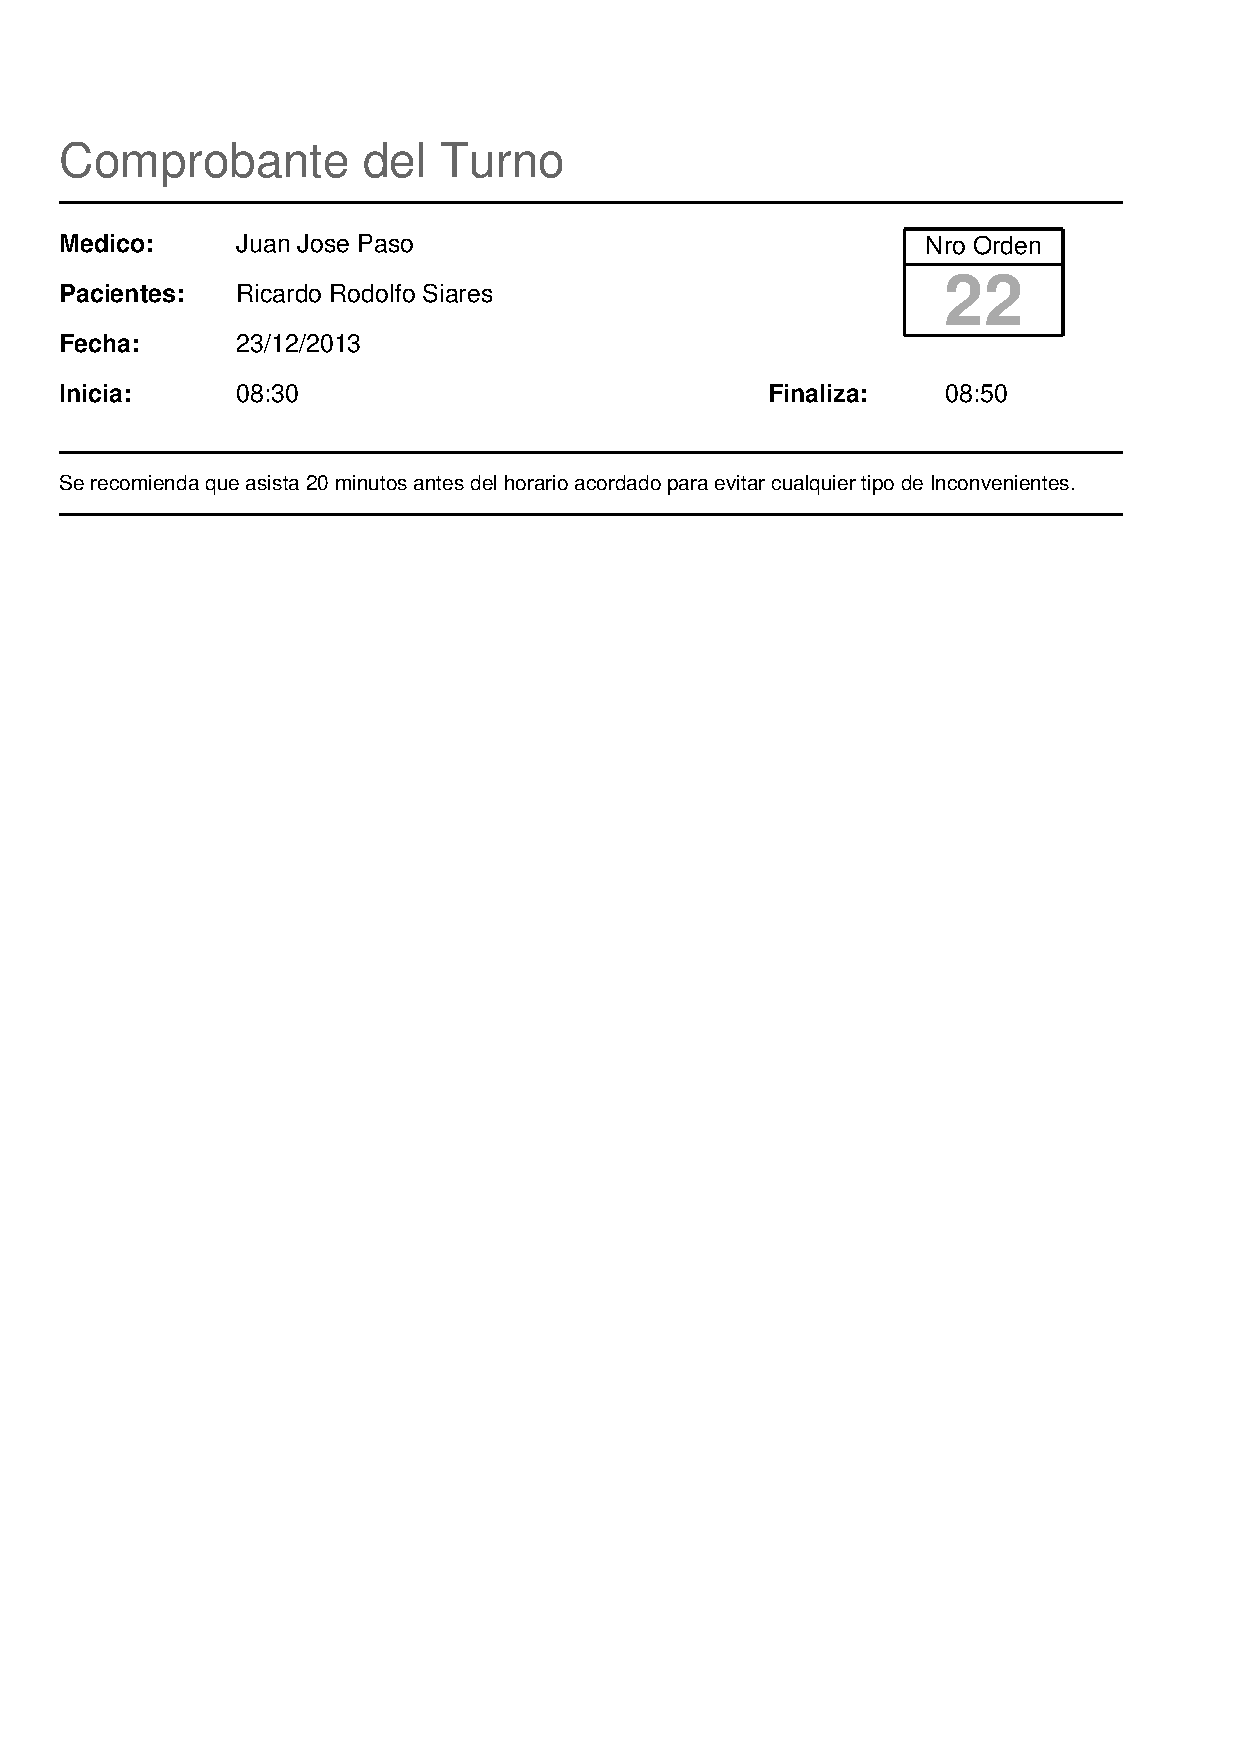
\includegraphics[scale=0.5]{resourse/comprobante-turno.png}
    \caption{Ejemplo de Comprobante de turno}
    \label{fig:625}
\end{figure}

Con esto último, se concluye esta pequeña guía de uso del sistema.














\chapter{Conclusion y Mejoras}


\section{Resultado}

El Sistemas de Gestión de Consultorios Medico proporciona soporte para Gestión de Turnos para pacientes y médicos proveyendo una nueva manera de mejorar la comunicación entre el paciente y el médico atraves de Internet, Permite administrar las Historias Clínicas dejando de depender de archivos físicos y con la posibilidad de almacenar los mismos en la nube.\\[0.1cm]

Considero que se alcanzaron casi todos los objetivos planteados y otros no planteados en la etapa inicial.


\subsection{Ventajas Percibidas}

Las Ventajas y Desventajas en lo que respeta al sistema fueron expuestas en el \textit{Capítulo IV} cuando se realizo una comparación con el actual funcionamiento de la mayoría de las instituciones, aquí se analizan las relacionadas a las herramientas que se utilizaron en su desarrollo.

\begin{itemize}
    \item La primera ventaja que encontré fue la velocidad de desarrollo comparando con otras herramientas aunque Python no es un 4GL sino un 3GL la facilidad de entendimiento de su sintaxis hace que el código
        sea fácilmente entendible y legible lo que permite un mantenimiento sencillo, el código en Python se asemeja mucho a lo que hacemos cuando escribimos un algoritmo en el papel por lo que la curva de aprendizaje si ya manejas algún lenguaje es mínima.

    \item Django y el Modelo de desarrollo MVC (Modelo Vista Controlador) aportaron otro extra a la velocidad de desarrollo del sistema ya que  solo con un par de líneas era capaz de crear vistas fácilmente adaptables, además de la característica de poder heredar plantillas por lo que en caso que quisiera realizar un cambio en el diseño de la plantilla solo requería cambiar la plantilla maestra o base sin necesidad de estar modificando una por una todas las plantillas, ni hablar si el código hubiese estado mesclado con el HTML como ocurre       aveces con PHP por ejemplo.

    \item Otra característica interesante de Django que me ahorro sufrimiento fue la definición de Modelos, cuando trabajas con Django no hace falta conocer el motor de Base de Datos y su sintaxis, no te debes preocupar por aprender cómo realizar tal o cual consulta, dejas de pelear con los JOIN de SQL y demás, solo te dedicas a aprender a manejar el Object Relational Model o ORM que forma parte de Django el cual es         sencillo de aprender.

    \item Aunque no está relacionado en si con el desarrollo de manera explícita agradezco haber conocido sitios como url{http://www.stackoverflow.com} que es un sitio colaborativo donde podes hacer preguntas y/o responderlas sobre cuestiones de programación, instalaciones, errores, etc. Fue una gran ayuda ya que pude solucionar gracias a eso muchas de las dificultades y entender el problema de las mismas de manera rápida.

    \item Aprender a usar un sistema de control de versiones para el código fuente como GIT de mi proyecto fue de gran utilidad ya que el desarrollo de esta aplicación no fue de manera continua sino que variada durante todo el tiempo de desarrollo.
\end{itemize}


\subsection{Desventajas Percibidas}

No todo el desarrollo fue como se esperaba, surgieron una serie de inconvenientes o limitaciones relacionadas con la herramienta.

\begin{itemize}
    \item Hacer Deploy \footnote{Implementar un servidor de producción con Apache, Python, Django y PosgreSQl, mod\_wsgi} con la herramienta no es tan fácil como cuando instalas LAMP, pierdes mucho tiempo intentando configurar el servidor, la documentación existente sobre la misma es muy poca y normalmente incompleta.

    \item En su mayoría la documentación sobre las librerías y demás herramientas se encuentra escrita en ingles, no lo consideraría en si una desventaja pero lo menciono en este apartado por mi bajo nivel en lo que respecta a lectura y comprensión de texto en ingles.
\end{itemize}


\section{Futuras Mejoras}

El sistema podría evolucionar de varias maneras, al ser un sistema diseñado mediante plantillas la principal evolución del mismo es que se podría adaptar las interfaces a los navegadores de los dispositivos móviles inteligentes mediante un diseño responsive. \\[0.1cm]

Otra mejora común al sistema, seria que pueda integrarse con otros estudios como poder registrar análisis de laboratorio, odontograma, integración con  el sistema vademécum para que sea más sencillo elaborar una receta médica,  y la posibilidad de importar y/o exportar la historia clínica a formatos conocidos como archivos PDF para permitir ser exportado a papel.



%\part*{\addcontentsline{toc}{part}{Apéndices}Apéndices}

% Adjustments headers
%\fancyhead[RO]{\leftmark}
%\fancyhead[EL]{\emph{Apéndice \thechapter}}

%%%%%%%%%%%%%
%\appendix
%%%%%%%%%%%%%%
%\ include{software}
%\ include{publicaciones}
%\begin{thebibliography}{X}

    \bibitem{Apache} \textsc{Wikipedia} \textit{Servidor HTTP Apache} 
        http://es.wikipedia.org/wiki/Servidor\_HTTP\_Apache 

    \bibitem{ApacheUbuntu} \textit{Servidor Apache en Ubuntu} 
        http://kuyne.blogspot.com.ar/2013/03/servidor-apache-en-ubuntu-instalacion-y.html     

    \bibitem{ApacheWin} \textit{Servidor Apache en Windows} 
        http://norfipc.com/internet/instalar-servidor-apache.html

    \bibitem{MVC} \textsc{Wikipedia} \textit{El Modelo Vista Controlador}
        http://es.wikipedia.org/wiki/Modelo\_Vista\_Controlador

    \bibitem{Presc} \textsc{Rogelio León López, Bárbara Gallego Machado y José Díaz Novás} \textit{Formato recomendable para llenar la hoja de remisión médica de un paciente} 
        http://bvs.sld.cu/revistas/mgi/vol22\_2\_06/mgi10206.htm 

    \bibitem{ConWeb} \textsc{Sistema Consultorio Web} \textit{Registro Consulta}
        https://www.consultorioweb.com/intranet/doctor/pacienteConsultas.aspx
    
    \bibitem{PracHisClin} \textsc{PRACTICA FINAL OBLIGATORIA: INTERNADO ROTATORIO Y PASANTIA RURAL OBLIGATORIA} \textit{Modelo Historia Clinica} 
        http://www.med.unne.edu.ar/internado/his\_cli.pdf
    
    \bibitem{ModHistClin} \textsc{Any Flowers} \textit{Modelo Historia Clinica}
        http://www.slideshare.net/AnyFlowers/ejemplo-historia-clinica
    
    \bibitem{BiocomHistCLin} \textsc{Biocom} \textit{Formato de Historia Clinica}
        http://www.biocom.com/informatica\_medica/historia\_5\_examen\_fisico.html
    
    \bibitem{ExamReg} \textsc{Infomed Red de Salud de Cuba} \textit{Examen Fisico Regional} 
        http://www.sld.cu/galerias/pdf/sitios/pdguanabo/cap04.pdf
    
    \bibitem{ProbAudit} \textsc{ESMAS} \textit{Problemas Auditivos Comunes}
        http://www.esmas.com/salud/enfermedades/notransmisibles/368755.html
    
    \bibitem{PerdAudi} \textsc{Wikipedia} \textit{Perdida de Audicion}
        http://es.wikipedia.org/wiki/P\%C3\%A9rdida\_de\_audici\%C3\%B3n

    \bibitem{Rinolo} \textsc{Hernado Vargas Vásquez} \textit{Rinologia}
        http://sisbib.unmsm.edu.pe/BibVirtualdata/libros/Medicina/cirugia/Tomo\_V/archivos\%20PDF/7Rinologia.pdf
    
    \bibitem{Labio} \textsc{Wikipedia} \textit{Examen Labios} 
        http://es.wikipedia.org/wiki/Labio

    \bibitem{Receta} \textsc{Consumoteca} \textit{Qué partes deben tener y datos incluir por ley las recetas médicas}
        http://www.consumoteca.com/bienestar-y-salud/medicamentos/que-partes-deben-tener-y-datos-incluir-por-ley-las-recetas-medicas/

    \bibitem{Farmacos} \textsc{Wikipedia} \textit{Vias de Administracion de Farmacos}
        http://es.wikipedia.org/wiki/V\%C3\%ADas\_de\_administraci\%C3\%B3n\_de\_f\%C3\%A1rmacos
    
    \bibitem{Res} \textsc{Pontificia Universidad Catolica de Chile - Escuela de Medicina} \textit{Respiracion}
        http://escuela.med.puc.cl/Publ/ManualSemiologia/190Respiracion.htm

    \bibitem{FisiExam} \textsc{Biocom} \textit{Historia Clinica - Examen Fisico}
        http://www.biocom.com/informatica\_medica/historia\_5\_examen\_fisico.html

    \bibitem{SlideShare} \textit{Examen Fisico del Sistema Ostiomioarticular}
        http://www.slideshare.net/wendy1971/examen-fisico-del-sistema-ostiomioarticular
    
    \bibitem{ModWsgi} \textsc{ModWsgi} \textit{Guia de Configuracion}
        https://code.google.com/p/modwsgi/wiki/QuickConfigurationGuide
 
    \bibitem{WSGI} \textsc{WSGI} \textit{Guia de Referencia WSGI - EN} 
        http://wsgi.readthedocs.org/en/latest/
    
    \bibitem{Apachee} \textsc{Apache} \textit{URL Mapping} 
        http://httpd.apache.org/docs/2.2/urlmapping.html

    \bibitem{MSal} \textsc{Ministerio de Salud } \textit{Formato de Historia Clinica}
        http://msal.gov.ar/ENT/SRV/Materiales\_Paciente/Herramientas\_Utiles/Historia\_Clinica/Historia\_Clinica.aspx
   
    \bibitem{HistCLin} \textsc{Historia Clinica que es} 
        http://es.wikipedia.org/wiki/Historia\_cl%C3%ADnica

    \bibitem{SemioClin} \textsc{Sem\'{\i}ologia Clinica}
        http://es.wikipedia.org/wiki/Semiolog%C3%ADa\_cl%C3%ADnica

    \bibitem{LeyHC} \textsc{Ley 26.529} \textit{Normativa sobre el Manejo de Historia Clinica}
        http://www.msaludjujuy.gov.ar/Re2014/Archi\_Varios%5Cley_26529.pdf
    
    %\bibitem{} \textsc{} \textit{}
    %\bibitem{} \textsc{} \textit{}
    %\bibitem{} \textsc{} \textit{}
\end{thebibliography}


%%%%%%%%%%%%%
\backmatter
%%%%%%%%%%%%%
% Adjustments headers
\fancyhead[RO]{\leftmark}
\fancyhead[EL]{}
\addcontentsline{toc}{chapter}{Bibliografía}
%\bibliographystyle{unsrt}
%\bibliographystyle{plain}
%\bibliography{biblio.bib}

\include{bibligrafia}

\end{document}

%%% Local Variables: 
%%% mode: latex
%%% TeX-master: "tesis"
%%% End: 
